% MDPI Machines submission (article two-column, MDPI-style front matter)
\documentclass[10pt,a4paper,twocolumn]{article}

\usepackage[T1]{fontenc}
\usepackage[utf8]{inputenc}
\usepackage[margin=1.85cm,top=1.75cm,bottom=1.85cm,columnsep=0.7cm]{geometry}
\usepackage{amsmath,amssymb}
\usepackage{graphicx}
\graphicspath{{../figures/}{figures/}}
\usepackage{booktabs}
\usepackage{multirow}
\usepackage{array}
\usepackage{caption}
\usepackage[ruled,vlined,linesnumbered]{algorithm2e}
\SetKwComment{Comment}{$\triangleright$\ }{}
\usepackage{natbib}
\usepackage{hyperref}
\usepackage{lineno}
\linenumbers

% generated by src/make_macros.py, do not edit

\newcommand{\ablA}{0.65}
\newcommand{\ablB}{0.49}
\newcommand{\ablFull}{0.60}
\newcommand{\algebraicMis}{15.17 $\pm$ 12.24}
\newcommand{\ccCost}{1.8}
\newcommand{\chaosTauACF}{46.10\%}
\newcommand{\chaosTauCC}{66.45\%}
\newcommand{\chaosTauLPF}{11.12\%}
\newcommand{\chaosTauMI}{15.17\%}
\newcommand{\chaosTauSE}{10.82\%}
\newcommand{\chaosWinACF}{1}
\newcommand{\chaosWinCC}{0}
\newcommand{\chaosWinLPF}{1}
\newcommand{\chaosWinMI}{1}
\newcommand{\chaosWinSE}{2}
\newcommand{\clsMfptBest}{1.00}
\newcommand{\clsMfptBestName}{time-domain statistics}
\newcommand{\clsMfptHg}{0.92}
\newcommand{\clsMfptHgMI}{0.95}
\newcommand{\clsMfptHgMr}{0.96}
\newcommand{\clsMfptHgRaw}{0.91}
\newcommand{\clsMfptRawTd}{0.99}
\newcommand{\clsMfptRawVmd}{1.00}
\newcommand{\clsMfptVmd}{1.00}
\newcommand{\clsRotorBest}{1.00}
\newcommand{\clsRotorBestName}{spectral band energies}
\newcommand{\clsRotorHg}{0.79}
\newcommand{\clsRotorHgMI}{0.87}
\newcommand{\clsRotorHgMr}{0.95}
\newcommand{\clsRotorHgRaw}{0.81}
\newcommand{\clsRotorHgSE}{0.83}
\newcommand{\clsRotorVmd}{1.00}
\newcommand{\devLowADP}{29.8}
\newcommand{\devLowCURV}{61.1}
\newcommand{\devLowFIT}{6.2}
\newcommand{\devLowLPF}{21.9}
\newcommand{\devLowMI}{8.2}
\newcommand{\devLowPE}{73.8}
\newcommand{\devLowSE}{4.4}
\newcommand{\devZeroADP}{0.25}
\newcommand{\devZeroCURV}{24.75}
\newcommand{\devZeroFIT}{0.50}
\newcommand{\devZeroLPF}{0.59}
\newcommand{\devZeroMI}{7.25}
\newcommand{\devZeroPE}{67.97}
\newcommand{\devZeroSE}{3.22}
\newcommand{\dispCleanLPF}{0.22}
\newcommand{\dispCleanMI}{2.44}
\newcommand{\dispCleanSE}{1.01}
\newcommand{\dispFiveLPF}{0.37}
\newcommand{\dispFiveMI}{3.59}
\newcommand{\dispFiveSE}{1.35}
\newcommand{\dispLowADP}{52.63}
\newcommand{\dispLowCURV}{52.98}
\newcommand{\dispLowFIT}{31.82}
\newcommand{\dispLowLPF}{50.31}
\newcommand{\dispLowMI}{1.18}
\newcommand{\dispLowPE}{31.44}
\newcommand{\dispLowSE}{1.10}
\newcommand{\dispTenLPF}{0.41}
\newcommand{\dispTenMI}{2.61}
\newcommand{\dispTenSE}{1.21}
\newcommand{\dispZeroADP}{0.62}
\newcommand{\dispZeroCURV}{22.97}
\newcommand{\dispZeroFIT}{1.38}
\newcommand{\dispZeroLPF}{0.61}
\newcommand{\dispZeroMI}{1.92}
\newcommand{\dispZeroPE}{15.40}
\newcommand{\dispZeroSE}{1.39}
\newcommand{\domCost}{0.4}
\newcommand{\domStage}{community detection}
\newcommand{\lleErrLPF}{40.5\%}
\newcommand{\lleErrSE}{27.0\%}
\newcommand{\lpfCost}{0.06}
\newcommand{\mechCvAccACF}{\textsc{tbd}}
\newcommand{\mechCvAccCC}{0.65}
\newcommand{\mechCvAccLPF}{0.60}
\newcommand{\mechCvAccMI}{0.80}
\newcommand{\mechCvAccSE}{0.74}
\newcommand{\mechHedgeMax}{24.3}
\newcommand{\mechHedgeMin}{10.4}
\newcommand{\mrBestLevel}{0.62}
\newcommand{\mrCombined}{0.81}
\newcommand{\nClassNames}{the four measured states}
\newcommand{\nMfptClasses}{three bearing states}
\newcommand{\nMfptPerClass}{45}
\newcommand{\nMfptPts}{2048}
\newcommand{\nMfptSignals}{135}
\newcommand{\nPerClass}{45}
\newcommand{\nPts}{2048}
\newcommand{\nSignals}{180}
\newcommand{\nSystems}{5}
\newcommand{\niFast}{0.42}
\newcommand{\niRef}{4.71}
\newcommand{\niSpeedup}{11}
\newcommand{\noiseRelCC}{31.3\%}
\newcommand{\noiseRelLPF}{20.7\%}
\newcommand{\noiseRelLowCC}{55.4\%}
\newcommand{\noiseRelLowLPF}{232.2\%}
\newcommand{\noiseRelLowMI}{78.9\%}
\newcommand{\noiseRelLowSE}{77.1\%}
\newcommand{\noiseRelMI}{71.6\%}
\newcommand{\noiseRelSE}{54.6\%}
\newcommand{\pipeTime}{0.7}
\newcommand{\propAccCleanLPF}{0.650}
\newcommand{\propAccCleanMI}{0.767}
\newcommand{\propAccCleanSE}{0.717}
\newcommand{\propAccFifteenLPF}{0.511}
\newcommand{\propAccFifteenMI}{0.767}
\newcommand{\propAccFifteenSE}{0.617}
\newcommand{\propAccFiveLPF}{0.572}
\newcommand{\propAccFiveMI}{0.672}
\newcommand{\propAccFiveSE}{0.639}
\newcommand{\propAccTenLPF}{0.561}
\newcommand{\propAccTenMI}{0.661}
\newcommand{\propAccTenSE}{0.661}
\newcommand{\propDispCleanLPF}{0.22}
\newcommand{\propDispCleanMI}{2.44}
\newcommand{\propDispCleanSE}{1.01}
\newcommand{\propDispFifteenLPF}{0.38}
\newcommand{\propDispFifteenMI}{2.34}
\newcommand{\propDispFifteenSE}{0.89}
\newcommand{\propDispFiveLPF}{0.36}
\newcommand{\propDispFiveMI}{3.47}
\newcommand{\propDispFiveSE}{1.27}
\newcommand{\propDispTenLPF}{0.37}
\newcommand{\propDispTenMI}{2.32}
\newcommand{\propDispTenSE}{1.20}
\newcommand{\propMrCleanLPF}{0.811}
\newcommand{\propMrCleanSE}{0.789}
\newcommand{\propMrTenLPF}{0.653}
\newcommand{\propMrTenSE}{0.619}
\newcommand{\rotorNoiseCC}{18.6}
\newcommand{\rotorNoiseLPF}{0.7}
\newcommand{\rotorNoiseLowCC}{18.5}
\newcommand{\rotorNoiseLowLPF}{28.2}
\newcommand{\rotorNoiseLowMI}{8.5}
\newcommand{\rotorNoiseLowSE}{4.3}
\newcommand{\rotorNoiseMI}{7.0}
\newcommand{\rotorNoiseSE}{3.3}
\newcommand{\rotorTauStdACF}{1.54}
\newcommand{\rotorTauStdCC}{13.12}
\newcommand{\rotorTauStdLPF}{0.22}
\newcommand{\rotorTauStdMI}{2.32}
\newcommand{\rotorTauStdSE}{0.97}
\newcommand{\sensCvSpan}{0.12}
\newcommand{\sensTauSpan}{12}
\newcommand{\sepAdaptive}{0.939}
\newcommand{\sepAdaptiveGain}{0.006}
\newcommand{\sepCleanADP}{0.889}
\newcommand{\sepCleanCURV}{0.806}
\newcommand{\sepCleanFIT}{0.939}
\newcommand{\sepCleanLPF}{0.561}
\newcommand{\sepCleanMI}{0.772}
\newcommand{\sepCleanPE}{0.656}
\newcommand{\sepCleanSE}{0.744}
\newcommand{\sepDispCleanADP}{0.12}
\newcommand{\sepDispCleanCURV}{0.12}
\newcommand{\sepDispCleanFIT}{0.12}
\newcommand{\sepDispCleanLPF}{0.18}
\newcommand{\sepDispCleanMI}{2.37}
\newcommand{\sepDispCleanPE}{0.22}
\newcommand{\sepDispCleanSE}{1.03}
\newcommand{\sepDispTenADP}{0.19}
\newcommand{\sepDispTenCURV}{10.34}
\newcommand{\sepDispTenFIT}{0.32}
\newcommand{\sepDispTenLPF}{0.33}
\newcommand{\sepDispTenMI}{2.33}
\newcommand{\sepDispTenPE}{11.33}
\newcommand{\sepDispTenSE}{1.13}
\newcommand{\sepFixTen}{0.539}
\newcommand{\sepFixTwo}{0.933}
\newcommand{\sepLowADP}{0.367}
\newcommand{\sepLowCURV}{0.356}
\newcommand{\sepLowFIT}{0.367}
\newcommand{\sepLowLPF}{0.340}
\newcommand{\sepLowMI}{0.281}
\newcommand{\sepLowPE}{0.406}
\newcommand{\sepLowSE}{0.367}
\newcommand{\sepNormADP}{0.894}
\newcommand{\sepNormCURV}{0.817}
\newcommand{\sepNormFIT}{0.939}
\newcommand{\sepNormLPF}{0.578}
\newcommand{\sepNormMI}{0.761}
\newcommand{\sepNormPE}{0.656}
\newcommand{\sepNormSE}{0.750}
\newcommand{\sepPeakTau}{2}
\newcommand{\sepTenADP}{0.677}
\newcommand{\sepTenCURV}{0.739}
\newcommand{\sepTenFIT}{0.694}
\newcommand{\sepTenLPF}{0.604}
\newcommand{\sepTenMI}{0.636}
\newcommand{\sepTenPE}{0.665}
\newcommand{\sepTenSE}{0.632}
\newcommand{\sepZeroADP}{0.573}
\newcommand{\sepZeroCURV}{0.447}
\newcommand{\sepZeroFIT}{0.535}
\newcommand{\sepZeroLPF}{0.523}
\newcommand{\sepZeroMI}{0.544}
\newcommand{\sepZeroPE}{0.843}
\newcommand{\sepZeroSE}{0.568}
\newcommand{\snrLow}{-5}
\newcommand{\snrMid}{0}
\newcommand{\tauScaleADP}{4.6}
\newcommand{\tauScaleCURV}{6.6}
\newcommand{\tauScaleFIT}{2.3}
\newcommand{\tauScaleLPF}{10.8}
\newcommand{\tauScaleMI}{10.5}
\newcommand{\tauScalePE}{12.4}
\newcommand{\tauScaleSE}{7.5}
\newcommand{\varNoiseACF}{14.7\%}
\newcommand{\varNoiseADP}{10.5\%}
\newcommand{\varNoiseCC}{31.2\%}
\newcommand{\varNoiseCURV}{337.1\%}
\newcommand{\varNoiseFIT}{11.5\%}
\newcommand{\varNoiseLPF}{14.6\%}
\newcommand{\varNoiseMI}{17.2\%}
\newcommand{\varNoisePE}{200.3\%}
\newcommand{\varNoiseSE}{42.1\%}
\newcommand{\varRatioACF}{6.3}
\newcommand{\varRatioADP}{1.6}
\newcommand{\varRatioCC}{3.2}
\newcommand{\varRatioCURV}{1.9}
\newcommand{\varRatioFIT}{2.5}
\newcommand{\varRatioLPF}{0.6}
\newcommand{\varRatioMI}{2.0}
\newcommand{\varRatioPE}{4.3}
\newcommand{\varRatioSE}{1.3}
\newcommand{\varRotorNoiseACF}{0.7}
\newcommand{\varRotorNoiseADP}{0.0}
\newcommand{\varRotorNoiseCC}{18.2}
\newcommand{\varRotorNoiseCURV}{20.9}
\newcommand{\varRotorNoiseFIT}{0.3}
\newcommand{\varRotorNoiseLPF}{0.4}
\newcommand{\varRotorNoiseMI}{2.0}
\newcommand{\varRotorNoisePE}{75.2}
\newcommand{\varRotorNoiseSE}{1.0}
\newcommand{\varRotorStdACF}{5.64}
\newcommand{\varRotorStdADP}{0.48}
\newcommand{\varRotorStdCC}{29.50}
\newcommand{\varRotorStdCURV}{0.49}
\newcommand{\varRotorStdFIT}{0.46}
\newcommand{\varRotorStdLPF}{0.40}
\newcommand{\varRotorStdMI}{5.08}
\newcommand{\varRotorStdPE}{2.31}
\newcommand{\varRotorStdSE}{1.53}
\newcommand{\varTauACF}{46.10\%}
\newcommand{\varTauADP}{57.88\%}
\newcommand{\varTauCC}{66.45\%}
\newcommand{\varTauCURV}{52.81\%}
\newcommand{\varTauFIT}{66.37\%}
\newcommand{\varTauLPF}{11.12\%}
\newcommand{\varTauMI}{15.17\%}
\newcommand{\varTauPE}{57.19\%}
\newcommand{\varTauSE}{10.82\%}

\newcommand{\lpf}{\textsc{lpf-sem}}
\newcommand{\nilouvain}{\textsc{ni-louvain}}

\begin{document}

%=================================================================
% Title page (single column across the whole width)
%=================================================================
\twocolumn[\begin{center}
{\LARGE\bfseries Saturated Symbolic Entropy Phase-Space Reconstruction and NI-Louvain Driven Multi-Resolution Hypergraph Modelling for Rotor Fault Time-Series Characterisation\par}
\vspace{0.6em}
{\normalsize Zhenmin~Zhao$^{1}$, Jianghong~Li$^{2,3,*}$ and Jiahang~Cui$^{2}$\par}
\vspace{0.3em}
{\footnotesize $^{1}$ National Elite Institute of Engineering, Northwestern Polytechnical University, Xi'an 710072, China\par}
{\footnotesize $^{2}$ School of Power and Energy, Northwestern Polytechnical University, Xi'an 710072, China\par}
{\footnotesize $^{3}$ Science and Technology on Altitude Simulation Laboratory, Northwestern Polytechnical University, Xi'an 710072, China\par}
\vspace{0.3em}
{\footnotesize * Correspondence: jhli@nwpu.edu.cn\par}
\vspace{0.6em}
\end{center}]

\noindent\textbf{\textit{Abstract:}} Phase-space reconstruction supplies the geometric foundation of nonlinear vibration analysis, yet its delay parameter is sensitive to the impulsive glitches and local extrema that pervade measured rotor signals, while graph-based descriptions rarely move beyond pairwise edges even though a fault state is naturally a relation among many interacting points. This paper builds an interpretable, training-free hypergraph framework around three constructions. First, an NI-Louvain construction turns a recurrence graph into a hypergraph through overlapping communities, each community becoming one hyperedge so that the higher-order coupling of the series is represented explicitly; an ablation shows this step carries the separability, which falls from 0.60 to 0.49 when it is removed. Second, a variational mode decomposition multi-resolution framework runs the chain per intrinsic mode function, yielding a combined descriptor of 0.81 against 0.62 for the best single level. Third, a saturated symbolic entropy estimator smooths the entropy curve with a low-pass filter and reads the delay at the rapid-to-saturated junction; it is not the more accurate estimator on the clean benchmark, but the more stable and noise-robust one; a controlled sweep shows the downstream separability is a unimodal function of the delay peaked at the small-lag recurrence window, and the estimator's job is to land reliably inside that window rather than to read an accurate delay, so the saturated rule is valued for its stability and robustness. Validated on five chaotic systems, 180 measured rotor signals covering the four measured states, and the public MFPT bearing set, the framework is a training-free, interpretable alternative to learned classifiers on small rotor record sets.\\[0.4em]
\noindent\textbf{\textit{Keywords:}} rotor fault diagnosis; phase-space reconstruction; symbolic entropy; low-pass filtering; recurrence network; overlapping community; hypergraph; variational mode decomposition; multi-resolution analysis

\section{Introduction}
\label{sec:intro}

Rotating machinery faults leave their signature in the geometry of the
vibration signal.  A rub-impact, an unbalance or a misalignment does not only
change the amplitude of a few frequency lines; it changes the way the
trajectory of the system folds onto itself in phase space.  This is why
nonlinear time-series methods, and in particular phase-space reconstruction
(PSR) in the sense of Takens \citep{takens1981} and Packard et al.
\citep{packard1980}, have been repeatedly brought into fault diagnosis, in
bearing diagnostics \citep{randall2011,antoni2007,smith2015} and in rotor
diagnosis \citep{zhao2025}.  The general methodology is set out in standard
monographs \citep{kantz2004,schreiber1999}.  The
appeal of PSR is that it converts a scalar record into a trajectory whose
geometry, and whose derived invariants such as the largest Lyapunov exponent
\citep{rosenstein1993} or the correlation dimension
\citep{grassberger1983}, can be related to physical mechanisms.  The
difficulty of PSR is that the trajectory is only as good as the two
parameters that define it, namely the delay $\tau$ and the embedding
dimension $m$.

\subsection{Delay and dimension selection}

Forty years of work have produced a small catalogue of delay selection rules.
The autocorrelation function reaches $1/e$ at a characteristic delay
\citep{abarbanel1996}, the average mutual information is minimised at a
first minimum \citep{fraser1986}, the C-C method of Kim, Eykholt and Salas
\citep{kim1999} combines a delay statistic with an embedding-window
statistic, and the embedding dimension is most often fixed by the
false-nearest-neighbour criterion of Kennel et al. \citep{kennel1992} or by
Cao's practical variant \citep{cao1997}.  Symbolic entropy occupies a
special place among these rules because it is defined directly on the
phase-space vectors rather than on the scalar record
\citep{shannon1948,daw2003,bandt2002}.  Entropy measures more broadly, from
sample entropy \citep{richman2000} to multiscale entropy \citep{costa2002},
form a standard part of the complexity toolkit, and their use in machine
condition monitoring is well established \citep{minhas2021}.  The idea is to partition each
delay vector into a short symbol word according to whether its coordinates
fall above or below an amplitude threshold, and to select the delay at which
the entropy of the resulting symbol distribution stops changing quickly.  The
entropy curve as a function of the delay is therefore an information-theoretic
version of the autocorrelation criterion.

The symbolic rule has an obvious weakness that has received little attention
in the rotor literature.  The entropy curve computed on a real signal is not
smooth.  It is a sample statistic, and in a noisy, quasi-periodic record it
carries local extrema at nearly every delay.  A rule that selects the first
local maximum, which is the classical recipe, therefore latches onto a
fluctuation rather than onto a structural property of the signal.  The same
objection applies with less force to the autocorrelation and mutual
information criteria, which is why those criteria are sometimes preferred in
practice, but they in turn are known to overshoot when the signal contains
strong periodic components.  The first problem addressed here is therefore
narrow and concrete.  The symbolic entropy curve of a measured rotor signal
should be regularised before a delay is read from it, and the delay should be
read at a physically meaningful location rather than at the first extremum.
Section~\ref{sec:lpf} develops a low-pass filtered saturated symbolic entropy
estimator, abbreviated \lpf, that does exactly this.

\subsection{From pairwise graphs to hypergraphs}

The second gap concerns the object that the reconstructed trajectory is
mapped onto.  Two decades of work have shown that a time series can be turned
into a network and that the resulting topology carries dynamical information
\citep{zhang2006,xu2008,donner2010}.  Recurrence plots
\citep{eckmann1987,marwan2007} provide the most direct route, and recurrence
networks have since become a standard tool for classifying and monitoring
nonstationary signals.  In mechanical fault diagnosis the same idea has been
implemented repeatedly, for instance by converting bearing vibration into a
recurrence graph and feeding it to a graph neural network
\citep{yuan2023sen,yuan2023}.  All of these constructions are pairwise.  A
node is either adjacent to another node or it is not, and the resulting graph
expresses a relation between two phase-space points at a time.

A fault state, however, is a joint property of many points.  Unbalance
manifests as a coherent drift of an extended set of vectors; rub-impact
manifests as a recurrent excursion of a group of vectors towards a boundary.
Higher-order representations, hypergraphs and simplicial complexes, were
introduced precisely to express such group relations
\citep{berge1973,battiston2020,battiston2021}, and they have proved
productive in network science, from higher-order clustering
\citep{benson2016} through hypergraph learning \citep{zhou2006,feng2019} to
higher-order contagion \citep{iacopini2019}.  Within fault diagnosis the
hypergraph idea has begun to appear only recently, and almost always as a
component of a learned classifier, for example a multiresolution hypergraph
neural network \citep{yan2022}, a multisensor hypergraph fusion network
\citep{yan2024}, a deep hypergraph autoencoder \citep{shi2023} or a
multi-structure fusion projection \citep{su2023}.  What is missing is a
construction that is adapted to a one-dimensional vibration record and that
does not require training.  Section~\ref{sec:nilouvain} proposes to build the
hyperedges from overlapping communities, so that a phase-space point may
belong to several hyperedges and the multivariate coupling is represented
without a learning stage.

\subsection{Multi-resolution analysis of coupled faults}

The third gap is specific to coupled faults.  When a rotor rubs and is
simultaneously unbalanced, the measured signal is a superposition of
mechanisms whose characteristic time scales differ, and a single embedding
cannot represent all of them at once.  The established remedy in signal
processing is to decompose the record into narrow-band modes before any
nonlinear analysis, with the empirical mode decomposition
\citep{huang1998,lei2013} or with variational mode decomposition (VMD)
\citep{dragomiretskiy2014,wang2015vmd} as the two common choices.  VMD has
the advantage of a firm variational formulation and of a controllable mode
count.  Building descriptors at several scales is also related to multilayer
and multiscale network analysis, in which a system is represented by a family
of coupled layers rather than by a single graph \citep{boccaletti2014}.
Section~\ref{sec:vmd} therefore executes the whole chain, PSR then
recurrence network then hypergraph, separately on each intrinsic mode
function, and fuses the resulting descriptors.  The intent is not to claim a
complete decoupling of coupled faults, which would require more than a
decomposition, but to show which scales carry which part of the higher-order
structure and to establish a scope boundary for the method.

\subsection{Contributions and organisation}

The contributions of the paper are as follows.

\begin{enumerate}
\item An \nilouvain{} hypergraph construction for vibration time series.  A
recurrence graph is sparsified, its maximal cliques are enumerated, and
Louvain clustering of the clique graph yields overlapping communities that
become hyperedges.  The construction captures multivariate higher-order
coupling that a pairwise graph cannot express, and it is the design choice the
data support most directly: removing the overlap costs more separability than
any other single substitution tested.
(Section~\ref{sec:nilouvain}, Experiments~3 and~5.)
\item A VMD multi-resolution hypergraph framework.  The chain is executed per
mode, a concatenated multi-resolution descriptor is formed, and the evolution
of hyperedge size, hyperedge interaction and network connectivity across
scales is reported.  The framework is demonstrated on the measured states and
on a clearly labelled numerical coupling study.
(Section~\ref{sec:vmd}, Experiment~4.)
\item A saturated symbolic entropy PSR estimator, positioned as a stable and
robust front-end that feeds the hypergraph construction.  The symbolic
entropy curve is low-pass filtered with a Butterworth filter and the optimal
delay is taken at the junction between the rapid-change and saturated regimes,
located by a derivative threshold.  The estimator is validated on five chaotic
systems against four established baselines and on a set of measured rotor
signals, its robustness to additive noise and to impulsive glitches is
quantified, and the junction-location family to which it belongs is compared
against three refinements, so that the accuracy and stability of the reading
are stated precisely.  The result is reported as a stability, robustness and
cost gain rather than an accuracy gain, because the benchmark shows the two
entropy rules to be essentially tied on clean data and the junction refinements
to leave that reading unchanged; it is a stable, cheap way to fix the delay
rather than an accuracy improvement.  Read at the saturation time constant
$\tau_c$ rather than at the shoulder, the same front-end is also the most
separable delay in the paper, so the saturation scale is both stable and the
one the descriptor can use.
(Section~\ref{sec:lpf}, Experiments~1,~2,~8,~9 and~10.)
\end{enumerate}

Two features of the study should be stated at the outset, because they
constrain how the results should be read.  The work is a study of signal
preprocessing and hypergraph construction, not of machine learning.  No
classifier is proposed and no accuracy record is claimed for the method itself.
The separability indices reported below, a Kruskal-Wallis statistic, a
Fisher-type variance ratio and a nearest-centroid cross-validated index, are
used to compare feature sets on the same footing and to decide whether a
topology actually changes with the fault state.  Experiment~7 does apply three
off-the-shelf classifiers, but only as a fixed yardstick carried across every
representation in the comparison, so that the pipeline and not the model is
what varies.  In addition, of the eight fault states available in the source
data, four are measured directly and four are arithmetic means of pairs or
triples of the measured states.  The latter are treated throughout as a
numerical secondary study and are never allowed to carry a conclusion that the
measured states could not carry on their own.

The remainder of the paper is organised as follows.
Section~\ref{sec:theory} collects the necessary theory, including an explicit
account of why the original symbolic entropy rule fails.
Section~\ref{sec:method} develops the proposed methodology and its
complexity.  Section~\ref{sec:exp} reports the ten experiment groups, the
first six characterising the estimator, the topology, the multi-resolution
framework, the ablation and the cost, the seventh placing the representation
against mainstream feature pipelines on two datasets, the eighth testing
whether the delay stability propagates into the descriptor, the ninth
comparing the junction-location family of the estimator against three
refinements at the estimator level, and the tenth asking whether the delay
scale itself reaches the downstream separability.
Section~\ref{sec:disc} discusses what the results do and do not support, and
Section~\ref{sec:concl} concludes.

\begin{figure*}[t]
\centering
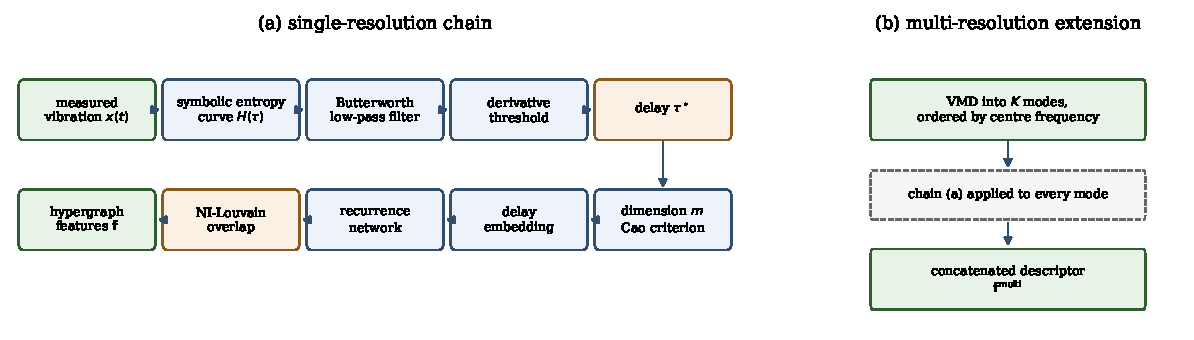
\includegraphics[width=0.95\textwidth]{fig1_pipeline.pdf}
\caption{The proposed pipeline.  The first two rows are the single-resolution
chain of Sections~\ref{sec:lpf} to \ref{sec:nilouvain}, from the record to
the hypergraph descriptor; the shaded boxes mark the two proposed steps.
The dashed row is the multi-resolution extension of Section~\ref{sec:vmd},
which applies the same chain to every intrinsic mode function and then
concatenates the descriptors.}
\label{fig:pipeline}
\end{figure*}

%==========================================================================
\section{Theoretical preliminaries}
\label{sec:theory}

\subsection{Time-delay embedding}

Let $x_1,\dots,x_N$ be a scalar record.  The delay embedding with delay
$\tau$ and dimension $m$ maps it to the vectors
\begin{equation}
\mathbf{x}_i = \bigl(x_i,\, x_{i+\tau},\, \dots,\, x_{i+(m-1)\tau}\bigr),
\qquad i = 1,\dots,N-(m-1)\tau .
\label{eq:embed}
\end{equation}
Takens' theorem \citep{takens1981} guarantees that for $m$ large enough the
map $\mathbf{x}_i \mapsto$ the underlying state is an embedding, so that the
delay vector reproduces the topology of the original attractor.  The theorem
is silent on how large $m$ must be and on which $\tau$ is admissible, which
is why the selection problem is empirical.  In what follows $\tau$ is always
reported in samples.  All delay estimates are therefore independent of the
assumed sampling rate, a point that is worth stating explicitly because it
removes an ambiguity in the testbed description from the interpretation of
the results.

\subsection{Symbolic entropy and the failure of the first-maximum rule}

The symbolic entropy of a delay vector is defined by first fixing an
amplitude threshold $e$ and a symbol length $p$.  Following the reference
implementation used in this work, $p=6$ and $e=1.2\,\sigma_x$, where
$\sigma_x$ is the standard deviation of the record.  Each delay vector is
encoded as a $(p-1)$-bit word.  The first coordinate decides the sense of the
comparison.  If $|v_0| < e$ the remaining bits record $|v_j| < e$; otherwise
they record $|v_j| \ge e$.  Writing the resulting integer code as $c_i$, the
symbol distribution is $P(c) = |\{i : c_i = c\}| / n$ and the symbolic
entropy is the Shannon entropy \citep{shannon1948}
\begin{equation}
H(\tau) = -\frac{1}{p}\sum_{c} P(c) \log P(c),
\label{eq:H}
\end{equation}
which is evaluated on a delay grid $\tau = 1,\dots,\tau_{\max}$ and
normalised by $p$ so that $H \in [0,1]$.

The classical rule selects the first local maximum of $H(\tau)$.  The rule
rests on an assumption that is rarely checked, namely that the curve rises
smoothly from a low value and then settles, so that its first local maximum
marks the transition from redundancy to saturation.  On a measured rotor
signal the assumption fails.  The curve of a single finite record is a
sample statistic and it fluctuates at the scale of the delay grid.  A local
maximum can then occur at a delay of a few samples purely by chance, and the
rule returns that fluctuation.  Figure~\ref{fig:entropy} contrasts the two
situations for three rub-impact records.  The unfiltered curves in
panel~(a) present extrema at almost every delay, and the first local maximum
is reached after only a few samples.  The corresponding delay vectors are
then strongly correlated and the reconstructed object is effectively
one-dimensional, which defeats the purpose of the embedding.  The remedy
developed in Section~\ref{sec:lpf} is to regularise the curve before the
delay is read.

\begin{figure*}[t]
\centering
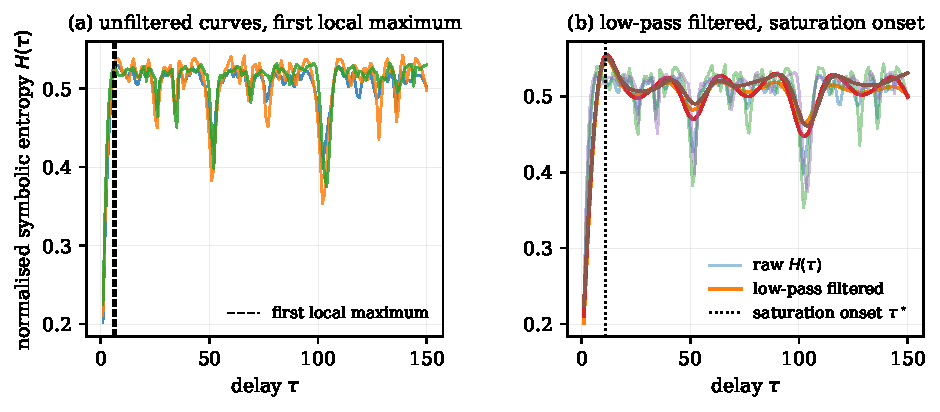
\includegraphics[width=0.95\textwidth]{fig2_entropy_curve.pdf}
\caption{The failure mechanism of the original symbolic entropy rule and the
behaviour of the saturated rule, for three measured rub-impact records.
(a) Unfiltered $H(\tau)$.  The curve fluctuates at the scale of the delay
grid, so the first local maximum (dashed) is a fluctuation rather than a
structural transition.  (b) The same curves after third-order Butterworth
low-pass filtering, with the saturation onset (dotted) located by the
derivative threshold rule of Eq.~\eqref{eq:tau_star}.}
\label{fig:entropy}
\end{figure*}

\subsection{Recurrence networks}

A recurrence plot \citep{eckmann1987,marwan2007} marks the pairs of times at
which the trajectory returns close to itself.  Given the threshold $\epsilon$,
the recurrence matrix is
\begin{equation}
R_{ij} = \Theta\bigl(\epsilon - \lVert \mathbf{x}_i - \mathbf{x}_j
\rVert\bigr), \qquad i,j = 1,\dots,n ,
\label{eq:rec}
\end{equation}
where $\Theta$ is the Heaviside step.  Reading $R$ as an adjacency matrix
turns the recurrence plot into a recurrence network
\citep{donner2010}, and the network invariants then describe the dynamics in
the language of complex networks
\citep{watts1998,barabasi1999,boccaletti2006}.  For pseudoperiodic signals a
recurrence network is a ring-like object, and earlier work has exploited its
topology to distinguish dynamical regimes \citep{zhang2006,xu2008}.  The
threshold is the one user choice in the construction.  It is set here as a
percentile of the pairwise distance distribution, which fixes the edge
density rather than the metric radius and therefore behaves comparably across
records of different amplitude.

\subsection{Overlapping communities and the modularity objective}

Community detection partitions the vertex set so that intra-community edges
are dense and inter-community edges are sparse
\citep{girvan2002,newman2004,newman2006,fortunato2010}.  The Louvain
algorithm \citep{blondel2008} maximises the modularity
\begin{equation}
Q = \frac{1}{2E}\sum_{ij}\Bigl(A_{ij} -
\frac{k_i k_j}{2E}\Bigr)\delta(c_i,c_j),
\label{eq:mod}
\end{equation}
where $E$ is the edge count and $k_i$ the degree of vertex $i$.  Louvain
returns a hard partition, in which a vertex belongs to exactly one community.
Overlapping structure is common in real networks and requires either a
dedicated method or a transformation.  The approach adopted here is what we
call \nilouvain{} (node-intersection Louvain): vertices are first expanded
into maximal cliques and the Louvain partition is computed on the clique
graph; a vertex that belongs to cliques assigned to different communities
thereby acquires several memberships \citep{palla2005,ahn2010}.  This is the
mechanism that produces overlap, and it is the reason the construction is
useful for a hypergraph.

\subsection{Variational mode decomposition}

VMD \citep{dragomiretskiy2014} writes a real signal as a sum of $K$ band
limited modes $u_k$ with centre frequencies $\omega_k$,
\begin{equation}
\min_{\{u_k\},\{\omega_k\}} \sum_{k=1}^{K}
\Bigl\lVert \partial_t\bigl[\bigl(\delta(t) +
\tfrac{j}{\pi t}\bigr)\ast u_k(t)\bigr] e^{-j\omega_k t}
\Bigr\rVert_2^2 ,
\quad \text{s.t.} \sum_k u_k = x ,
\label{eq:vmd}
\end{equation}
and solves it by alternating direction method of multipliers.  The two
parameters are the mode count $K$ and the bandwidth penalty.  Relative to the
empirical mode decomposition \citep{huang1998}, the recursive sifting
procedure is replaced by a single variational problem, which avoids mode
mixing and makes the decomposition reproducible for a fixed $K$.  Seeded
reconstruction experiments on the measured records, with $K=3$, leave a
residual of about half a percent of the signal energy, so the decomposition
is effectively lossless at that setting and can be used as the front end of a
nonlinear chain.

\subsection{Hypergraph representation}

A hypergraph $\mathcal{H} = (\mathcal{V},\mathcal{E})$ extends a graph by
allowing an edge, a hyperedge, to contain any number of vertices
\citep{berge1973}.  It is represented by an incidence matrix
$H \in \{0,1\}^{n \times k}$, with $H_{vj}=1$ when vertex $v$ belongs to
hyperedge $j$.  The vertex degree and hyperedge size are
\begin{equation}
d(v) = \sum_{j} H_{vj}, \qquad s(j) = \sum_{v} H_{vj} ,
\label{eq:degrees}
\end{equation}
and the higher-order coupling between two hyperedges is measured by the
Jaccard index
\begin{equation}
J(j,j') = \frac{|\mathcal{V}_j \cap \mathcal{V}_{j'}|}
{|\mathcal{V}_j \cup \mathcal{V}_{j'}|} .
\label{eq:jaccard}
\end{equation}
The mean of $J$ over hyperedge pairs, called hyperedge interaction below, is
the quantity that has no counterpart in a pairwise graph; it is large when
the group relations found by the construction overlap heavily.  The vertex
projection of the hypergraph is the adjacency
\begin{equation}
A^{(v)} = \bigl(H H^{\top} > 0\bigr) , \qquad
A^{(v)}_{vv} = 0 ,
\label{eq:projection}
\end{equation}
from which the ordinary connectivity diagnostics are read, including the
giant-component fraction, the algebraic connectivity, that is the second
smallest eigenvalue of the Laplacian, and the spectral entropy of the
leading eigenvalue spectrum.

%==========================================================================
\section{Proposed methodology}
\label{sec:method}

\subsection{Saturated symbolic entropy parameter estimation}
\label{sec:lpf}

The estimator replaces a single fragile criterion by a two-step procedure,
filter then threshold.

\paragraph{Step one, low-pass regularisation.}
The symbolic entropy curve of Eq.~\eqref{eq:H} is computed on the grid
$\tau=1,\dots,\tau_{\max}$ and passed through a third-order Butterworth
low-pass filter applied in both directions so that no phase shift is
introduced,
\begin{equation}
\widetilde{H}(\tau) = \mathrm{filtfilt}_{3,\,w_c}
\bigl[H(\tau)\bigr] ,
\label{eq:filt}
\end{equation}
with normalised cutoff $w_c = 0.1$.  The filter suppresses the sampling
fluctuations that Fig.~\ref{fig:entropy}(a) exposes while leaving the
underlying trend untouched.  Two remarks on the choice are in order.  The
order and the cutoff are not free in the sense that the delay estimate must
be stable against them, and Section~\ref{sec:exp2} reports the corresponding
sweep.  Applying the filter in both directions doubles the effective order
and, more importantly, avoids the group delay that a single forward pass
would superimpose on the curve, which would otherwise bias the delay
estimate by a fixed and signal-dependent amount.

\paragraph{Step two, derivative threshold.}
The regularised curve rises steeply while the embedding is redundant and then
flattens once the symbol distribution has saturated.  The junction between
the two regimes is located by the first derivative
\begin{equation}
\dot{H}(\tau) = \frac{\mathrm{d}\widetilde{H}}{\mathrm{d}\tau} ,
\label{eq:d1}
\end{equation}
whose maximum marks the steepest part of the rise.  Let
$\tau_p = \arg\max_{\tau} \dot{H}(\tau)$.  The optimal delay is the first
delay beyond $\tau_p$ at which the slope has fallen to a fixed fraction
$\alpha$ of its peak,
\begin{equation}
\tau^{\star} = \min\Bigl\{\tau > \tau_p \; : \;
\dot{H}(\tau) \le \alpha \, \dot{H}(\tau_p)\Bigr\} , \qquad \alpha = 0.1 .
\label{eq:tau_star}
\end{equation}
Equation~\eqref{eq:tau_star} is the formal statement of the derivative
threshold idea.  It has a direct physical reading.  Below $\tau^{\star}$ the
successive coordinates of a delay vector still carry redundant information,
because the symbolic word has not yet had time to explore the partition.
Beyond $\tau^{\star}$ the coordinates are effectively independent and the
word distribution has saturated, so no further delay adds information.  The
junction is where the marginal information gain per additional coordinate
becomes negligible, and $\alpha$ sets how conservatively that point is
declared.  A small $\alpha$ places $\tau^{\star}$ late, on the flat part of
the curve; a large $\alpha$ places it early, on the shoulder.  The sweep in
Section~\ref{sec:exp2} shows that the estimate moves slowly with $\alpha$
within a broad plateau, which is the empirical justification for fixing
$\alpha = 0.1$.

\paragraph{The junction-location family.}
The derivative threshold is one instance of a family of rules that all locate
the saturation onset of the filtered curve, and the choice among them is not
free of consequences, so the paper compares three alternatives and one change
of symbolisation in Experiment~9.  The first alternative locates the junction
at the point of maximum curvature, the direction of fastest change of the
curve,
\begin{equation}
\kappa(\tau) = \frac{\lvert \ddot{H}(\tau) \rvert}
{\bigl(1 + \bigl[\dot{H}(\tau)\bigr]^2\bigr)^{3/2}},
\qquad
\tau^{\star}_{\mathrm{curv}} = \arg\max_{\tau} \kappa(\tau) .
\label{eq:kappa}
\end{equation}
The curvature is low in the steep rise, where the slope is large but changes
slowly, and low again in the saturated tail, where the slope tends to zero; it
is largest at the transition itself, so Eq.~\eqref{eq:kappa} reads the
physical transition rather than a point on the flat tail.  The second
alternative fits a saturating exponential to the whole curve,
$H(\tau) \approx A\,(1 - e^{-\tau/\tau_c}) + B$, by nonlinear least squares,
and takes $\tau^{\star} = \tau_c$; it uses every point of the curve and gives
the transition a single characteristic scale.  The third alternative replaces
the fixed fraction $\alpha = 0.1$ by the value
$\alpha = \dot{H}(\tau_{\mathrm{mid}})/\dot{H}(\tau_p)$ computed at the
half-height crossing of the filtered curve, so that the declared junction
tracks the shape of the curve instead of a hard-coded fraction.  The fourth
change leaves the saturated-shoulder rule intact and replaces the symbolisation
by the standard ordinal-pattern (Bandt--Pompe) permutation entropy
\citep{bandt2002}, isolating the effect of the symbolisation on the delay.
Experiment~9 asks, for each of these, whether it changes the clean-benchmark
accuracy, the stability across records or the downstream separability of the
descriptor.

\paragraph{Embedding dimension.}
Once $\tau^{\star}$ is fixed, the embedding dimension is obtained from Cao's
false-nearest-neighbour criterion \citep{cao1997}, so that the estimator
supplies a complete parameter pair.  The criterion is used unchanged, because
the contribution of this paper concerns the delay; the dimension is reported
alongside the delay so that the downstream topology is fully specified.  The
original symbolic rule and the saturated rule share the same dimension
estimator, so the comparison between them isolates the delay rule.

The complete single-resolution chain is summarised in the upper row of
Fig.~\ref{fig:pipeline} and stated as pseudocode in
Algorithm~\ref{alg:pipeline}.

\begin{algorithm}[t]
\small
\caption{single-resolution hypergraph descriptor of one record}
\label{alg:pipeline}
\KwIn{record $x$, symbols $p$, threshold factor $e$, cutoff $w_c$,
threshold fraction $\alpha$, recurrence percentile $\rho$, removal ratio
$\pi$}
\KwOut{feature vector $\mathbf{f}$}
$H(\tau) \leftarrow$ symbolic entropy on $\tau = 1,\dots,\tau_{\max}$\Comment*{Eq.~\eqref{eq:H}}\;
$\widetilde{H} \leftarrow \mathrm{filtfilt}_{3,w_c}[H]$\Comment*{Eq.~\eqref{eq:filt}}\;
$\dot{H} \leftarrow \mathrm{d}\widetilde{H}/\mathrm{d}\tau$\;
$\tau_p \leftarrow \arg\max \dot{H}$\;
$\tau^{\star} \leftarrow \min\{\tau > \tau_p : \dot{H}(\tau) \le \alpha
\dot{H}(\tau_p)\}$\Comment*{Eq.~\eqref{eq:tau_star}}\;
$m \leftarrow$ Cao criterion at delay $\tau^{\star}$\Comment*{\citep{cao1997}}\;
$X \leftarrow$ delay embedding of $x$ with $(\tau^{\star}, m)$\Comment*{Eq.~\eqref{eq:embed}}\;
$\epsilon \leftarrow \rho$-th percentile of the pairwise distances in $X$\;
$R \leftarrow$ recurrence matrix at threshold $\epsilon$\Comment*{Eq.~\eqref{eq:rec}}\;
$R' \leftarrow$ remove fraction $\pi$ of the edges of $R$\;
$\mathcal{C} \leftarrow$ maximal cliques of $R'$\;
$G_c \leftarrow$ clique graph of $\mathcal{C}$\;
$\{c_v\} \leftarrow$ Louvain partition of $G_c$\Comment*{Eq.~\eqref{eq:mod}}\;
$\mathcal{E} \leftarrow$ vertex sets of the communities induced by $\{c_v\}$\Comment*{overlap allowed}\;
$\mathbf{f} \leftarrow$ features of $\mathcal{H} = (\mathcal{V},\mathcal{E})$\Comment*{Eqs.~\eqref{eq:degrees} to \eqref{eq:projection}}\;
\Return $\mathbf{f}$, $\tau^{\star}$, $m$
\end{algorithm}

\subsection{Recurrence graph construction}
\label{sec:recgraph}

The delay vectors of Eq.~\eqref{eq:embed} are treated as vertices.  The
pairwise Euclidean distance distribution is estimated from a random subsample,
and the recurrence threshold is its $\rho$-th percentile with $\rho = 5$.  The
subsample is required because the full distance matrix of a long record is
quadratic in memory, and the percentile of a subsample is a stable estimate
of the percentile of the whole.  The distance query itself is answered with a
spatial index, so that the edges can be recovered without ever materialising
the dense matrix.  Two consequences are worth recording.  The resulting
network is undirected and unweighted, because the threshold has already
encoded the metric information; and its edge density is controlled by $\rho$
rather than by the amplitude of the record, which is what makes the
construction transferable between signals measured on the same testbed.

\subsection{\nilouvain{} hypergraph construction}
\label{sec:nilouvain}

The recurrence network of a pseudoperiodic record is a nearly regular ring
with a very high edge density, and Louvain applied to it directly returns a
small number of large communities.  The \nilouvain{} construction interposes a
sparsification and a clique expansion, and it is this interposition that both
creates the overlap and sharpens the communities.

The steps are as follows and are also the body of
Algorithm~\ref{alg:pipeline}.  First, a fraction $\pi = 0.75$ of the edges is
removed at random while the vertex set is kept.  The removal is what breaks
the ring into locally dense patches.  Second, the maximal cliques of the
sparsified graph are enumerated.  Third, a clique graph is built whose
vertices are the cliques and whose edges join cliques that share a vertex of
the original graph.  Fourth, Louvain is applied to the clique graph, so that
cliques rather than vertices are clustered.  Fifth, the partition is mapped
back to the original vertices.  A vertex that belongs to cliques placed in
different communities receives several labels, and the communities so formed
overlap.  Each overlapping community is finally taken as one hyperedge, and
the incidence matrix of Eq.~\eqref{eq:degrees} is filled from those sets.

The construction has a clear interpretation for a vibration record.  A
maximal clique is a group of delay vectors that are mutually recurrent, that
is, a group of states that the system visits together.  Clustering the
cliques groups the mutually recurrent states into assemblies, and the overlap
records the fact that a single state can belong to two assemblies at once, for
example to a recurrent excursion and to a drift at the same time.  This is
precisely the multivariate relation that a pairwise graph cannot hold, and it
is why the hyperedge interaction of Eq.~\eqref{eq:jaccard} is informative.
The sparsification ratio $\pi$ is the principal knob of the construction, and
Section~\ref{sec:exp2} reports its effect on the downstream descriptor.

\subsection{VMD multi-resolution framework}
\label{sec:vmd}

The single-resolution chain answers a question about the whole record.  For a
coupled fault it is more informative to ask the same question at several
scales.  The record is decomposed by VMD into $K$ modes ordered by centre
frequency,
\begin{equation}
x(t) = \sum_{k=1}^{K} u_k(t) + r(t) ,
\label{eq:vmd_sum}
\end{equation}
and the chain of Algorithm~\ref{alg:pipeline} is executed on each $u_k$
independently, which means that every mode receives its own delay, its own
embedding and its own hypergraph.  Two descriptors are then available.  The
per-level descriptor $\mathbf{f}^{(k)}$ characterises the higher-order
structure that lives in the $k$-th band, and the concatenated descriptor
\begin{equation}
\mathbf{f}^{\mathrm{multi}} = \bigl[\mathbf{f}^{(1)}, \dots,
\mathbf{f}^{(K)}\bigr]
\label{eq:multidesc}
\end{equation}
characterises the record across scales.  Because the delay and the embedding
are re-estimated per mode, the levels are not required to share a common
geometry, which is the appropriate behaviour for a superposition of
mechanisms with different time scales.  The framework is stated in the lower
row of Fig.~\ref{fig:pipeline} and its cost is analysed next.

\subsection{Complexity}
\label{sec:complex}

The cost of the chain is dominated by two stages, and it is worth separating
them because they scale differently.  The symbolic entropy curve evaluates a
$(p-1)$-bit code for every delay vector at every delay on the grid, so its
cost is $O(\tau_{\max} N)$ and it is linear in the record length.  The
recurrence network requires the pairwise distances, a quadratic operation in
the number of vertices if it is written naively; the threshold estimation on
a fixed subsample and the spatial index used for the edge query reduce the
practical cost to a near-linear dependence on the vertex count, at the price
of the vertex cap that the construction applies when a record is very long.
The clique enumeration has no polynomial bound in the worst case, which is
the reason the sparsification is not merely a device for creating overlap but
also the mechanism that keeps the enumeration tractable on a dense
recurrence graph.  The remaining stages, the filter, the derivative, the
Louvain pass and the spectral diagnostics of a sparse projected graph, are
either linear or dominated by a few eigenpairs.  Experiment~6 measures the
actual constants, since the asymptotics alone do not say which stage a
practitioner should care about.

%==========================================================================
\section{Experimental validation}
\label{sec:exp}

\subsection{Data and setup}
\label{sec:setup}

\paragraph{Measured rotor signals.}
The measured data come from a scaled gas-turbine rotor testbed.  The set
contains \nSignals{} records, \nPerClass{} for each of \nClassNames{}, and
each record is \nPts{} samples long.  The states are a healthy baseline, a
rub-impact, an unbalance and a misalignment, all introduced physically on the
testbed.  The four measured states form the primary data set and every
conclusion below is drawn from them.

\paragraph{Measured bearing signals.}
The second data set is the public MFPT bearing set \citep{bechhoefer2013},
which supplies a different
machine, a different fault mechanism and a different sampling rate.  Three
conditions are used, a baseline and an inner-race and an outer-race fault, with
\nMfptPerClass{} records of \nMfptPts{} samples for each, \nMfptSignals{} in
all.  The source files are sampled at two rates; every record is decimated to
the lower rate so that the rate cannot act as a class cue.  The set is used
only in the classification comparison of Experiment~7.  It enters no other
experiment, and no conclusion about the estimator or about the topology is
drawn from it, because the recurrence graph of a bearing record is a different
object from that of a rotor record and the two should not be pooled.

\paragraph{Chaotic benchmark.}
Because a measured record has no ground truth for its delay, the estimator is
first characterised on five chaotic systems whose dynamics are known,
Lorenz, R\"ossler, Duffing, Mackey-Glass and Chen.  For each system a long
clean series is generated and the reference parameters are defined as the
median of the five estimators over that long series, which is the standard
consensus construction; the largest Lyapunov exponent is computed by the
Rosenstein method \citep{rosenstein1993} and compared with the literature
value to confirm that the reference is physically meaningful.

\paragraph{Baselines.}
Four established delay selectors are used throughout, the original symbolic
entropy rule with its first-local-maximum criterion, the average mutual
information with its first-minimum criterion \citep{fraser1986}, the
autocorrelation at a threshold of $1/e$ \citep{abarbanel1996} and the C-C
method \citep{kim1999}.  The embedding dimension is Cao's criterion
\citep{cao1997} for every method, so that a comparison between methods
isolates the delay rule.

\paragraph{Separability indices.}
Three descriptive quantities are used to compare feature sets.  The
Kruskal-Wallis statistic $H$ tests, feature by feature, whether the class
distributions differ.  A Fisher-type ratio compares the between-class to the
within-class variance and is averaged over features.  A nearest-centroid rule
under stratified cross-validation standardises the features on the training
fold and assigns each test sample to the closest class centroid.  The third
index is reported as a separability score and not as the accuracy of a
proposed classifier; the rule is deliberately elementary so that it measures
the geometry of the descriptor rather than the capacity of a model.  The
table of settings is given in Table~\ref{tab:setup}.

\begin{table*}[t]
\centering
\caption{Settings of the experiments.}
\label{tab:setup}
\small
\input{../tables/tab_setup.tex}
\end{table*}

\subsection{Experiment 1, phase-space reconstruction accuracy and robustness}
\label{sec:exp1}

\paragraph{Accuracy on the chaotic benchmark.}
Table~\ref{tab:chaos} reports the delay and dimension returned by every
method on the five systems, together with the reference pair, and
Table~\ref{tab:chaoserr} summarises the errors, which Fig.~\ref{fig:delay}(a,b)
shows as a bar chart.  On the clean benchmark the two entropy rules are
essentially tied.  The mean relative delay error is \chaosTauLPF{} for the
saturated rule against \chaosTauSE{} for the original symbolic rule, a
difference far smaller than the spread across systems, and the saturated rule
attains the smallest error on \chaosWinLPF{} of the \nSystems{} systems against
\chaosWinSE{} for the original rule and \chaosWinMI{} for the mutual
information criterion.  The largest Lyapunov exponent recovered from the
parameters is reproduced slightly less accurately by the saturated rule
(\lleErrLPF{} against \lleErrSE{}).  The scope of the contribution is fixed by
this reading.  On a long, clean, artefact-free series the original rule is not
impaired, because the local extrema it reads are themselves reliable, so the
saturated rule has no accuracy to recover.  One caveat applies to the
reference, which is the median of the five estimators and therefore lies by
construction inside the cluster formed by the entropy and information criteria,
making it a conservative yardstick for a rule of a different family.  The C-C
method is competitive on the delay, as expected because it also smooths a
statistic over an embedding window, but it is the weakest of the five on the
dimension, and the dimension errors of the entropy-based methods are comparable
because they share Cao's criterion.

\begin{table*}[t]
\centering
\caption{Reconstructed delay $\tau$ and embedding dimension $m$ for the five
chaotic systems.  The reference pair is the median of the five estimators on
a long clean series.}
\label{tab:chaos}
\scriptsize
\input{../tables/tab_chaos_est.tex}
\end{table*}

\begin{table*}[t]
\centering
\caption{Mean relative delay error and mean absolute dimension error of the
five selectors on the chaotic systems.}
\label{tab:chaoserr}
\scriptsize
\input{../tables/tab_chaos_err.tex}
\end{table*}

\paragraph{Estimates on the measured states.}
Table~\ref{tab:rotortau} lists the delay and dimension obtained for each
state, and Fig.~\ref{fig:delay}(c) shows the delay per state for the five
selectors.  The clearest result of the experiment is here, and it concerns
the stability of the delay rather than its accuracy, which on the measured
data has no reference to be measured against.  The saturated rule returns a
delay of about eleven samples for every state, with a standard deviation
averaged over the four states of \rotorTauStdLPF{}.  The original symbolic
rule returns a shorter delay of six to nine samples whose value drifts with
the state and whose spread is four times larger, \rotorTauStdSE{}.  The
mutual information and C-C criteria are less stable still, at
\rotorTauStdMI{} and \rotorTauStdCC{}.  The contrast is the one worth keeping
in mind.  A time delay is primarily a property of the sampling and of the
dominant time scales of the record rather than of the fault that is present,
so a delay estimate that is nearly the same for every state and has a small
spread across records is the behaviour a delay estimator should exhibit.  The
original rule's state dependence is a symptom of its failure mode, because it
reads the position of a local maximum of a raw sample statistic and that
position moves with the amplitude and with the transients of the signal.  The
saturated rule reads a smoothed shoulder and does not move.  Whether that
stability improves the descriptor built on top of the embedding is a separate
question, taken up in Experiments 3 and 8.

\begin{table*}[t]
\centering
\caption{Delay and embedding dimension estimated on the measured rotor
states, reported as mean and standard deviation over the records of each
state.}
\label{tab:rotortau}
\scriptsize
\input{../tables/tab_rotor_tau.tex}
\end{table*}

\begin{figure*}[t]
\centering
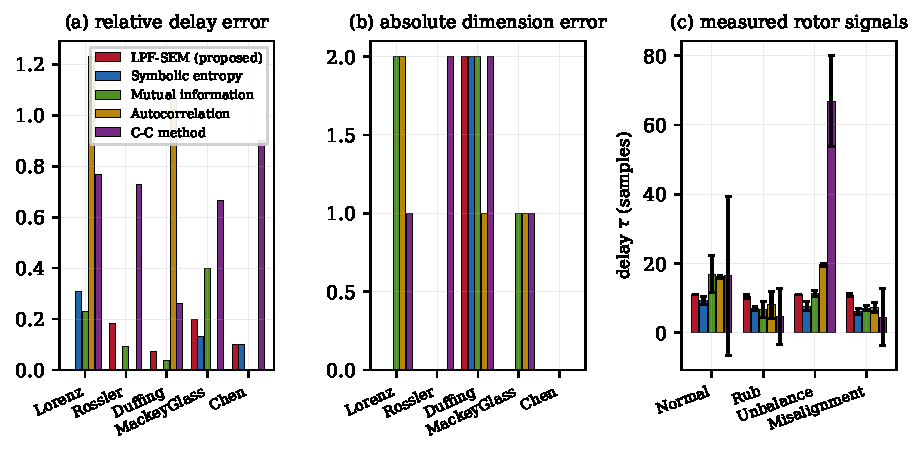
\includegraphics[width=0.95\textwidth]{fig3_delay_estimation.pdf}
\caption{Accuracy and stability of the delay estimate.  (a) Relative delay
error and (b) absolute dimension error on the five chaotic systems.  (c) Delay
estimate per measured rotor state, with the standard deviation over the
records of the state shown as an error bar.  On the measured records the
saturated rule returns a nearly state-independent delay with a small spread,
whereas the original symbolic rule returns a short delay that drifts with the
state.}
\label{fig:delay}
\end{figure*}

\paragraph{Robustness to additive noise.}
Figure~\ref{fig:robust} traces the delay error against the signal-to-noise
ratio.  Through the moderate regime the saturated estimator is the more
robust of the two rules.  At \snrMid{}~dB the mean relative error over the
chaotic systems is \noiseRelLPF{} for the saturated rule against
\noiseRelSE{} for the original symbolic rule, and the ordering is the same on
the measured records, where the mean absolute deviation is \rotorNoiseLPF{}
samples against \rotorNoiseSE{}.  The mechanism is the one argued in
Section~\ref{sec:theory}: noise perturbs the entropy curve pointwise, so a
criterion that reads a pointwise extremum is perturbed with it, whereas a
criterion that reads the position of a filtered shoulder averages the
perturbation away.  The advantage does not extend to the most severe noise
tested.  At \snrLow{}~dB the saturated rule degrades sharply and becomes the
worse of the two, \noiseRelLowLPF{} against \noiseRelLowSE{}, because the
filtered derivative that locates the shoulder is itself destroyed once the
noise dominates the curve.  The practical reading is that the saturated rule
should be preferred while the record retains a usable spectral signature, and
should not be trusted below the point at which it does not.

\begin{figure*}[t]
\centering
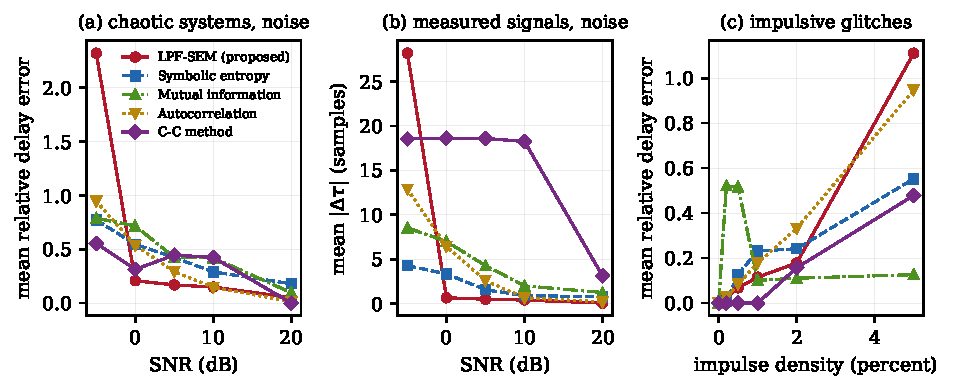
\includegraphics[width=0.95\textwidth]{fig4_robustness.pdf}
\caption{Robustness of the delay estimate.  (a) Mean relative error against
the signal-to-noise ratio over the five chaotic systems.  (b) Mean absolute
error against the signal-to-noise ratio on the measured rotor records.
(c) Mean relative error against the density of injected impulses, scaled to
the signal standard deviation and averaged over the five chaotic systems.}
\label{fig:robust}
\end{figure*}

\paragraph{Robustness to impulsive glitches.}
Figure~\ref{fig:robust}(c) adds impulses scaled to the signal standard
deviation at a controlled density.  This is the perturbation that matters most
in a rotor context, because a rub-impact produces exactly such transients.
The saturated estimator is the more stable of the two over the intermediate
densities tested, from roughly one impulse in two hundred samples to one in
fifty, where the filtered shoulder survives the transients.  It is not
uniformly better.  At the sparsest density tested a single isolated impulse
can displace the shoulder without displacing an extremum, and at the highest
density the original rule's shorter delay is the more robust quantity,
because it is set by the earliest extremum rather than by a broad feature.
The outcome is therefore a qualified form of the argument of
Section~\ref{sec:theory}, that a pointwise extremum of a sample statistic is a
fragile object, with the qualification that a smoothed feature becomes fragile
in a different way at the extremes of the perturbation range.

\subsection{Experiment 2, parameter sensitivity}
\label{sec:exp2}

The construction has five parameters, and they are of two kinds.  The filter
order, the cutoff and the threshold fraction act on the entropy curve and
therefore on the delay estimate; the removal ratio and the recurrence
percentile act on the downstream topology and are scored by separability
instead.  Table~\ref{tab:sens} reports both.

For the filter, the delay estimate is stable across orders two to five and
across cutoffs in the middle of the tested range, and it moves by only about
\sensTauSpan{} samples as the threshold fraction sweeps from $0.05$ to
$0.30$.  The estimator is therefore not balanced on a knife edge, which is
the property that matters for a practitioner, and the default settings sit in
the middle of the plateau.  For the topology, the separability score varies
by \sensCvSpan{} as the removal ratio sweeps the tested range, and the
default of $0.75$ is at or near the best observed value; the recurrence
percentile and the mode count behave similarly.  The pattern is that the
method has a broad operating region rather than a single tuned point, which
is the honest reading of a sweep of this kind.

\begin{table*}[t]
\centering
\caption{Parameter sensitivity.  The upper block reports the delay estimate
against the filter parameters, the lower block the downstream separability
score against the topology parameters.}
\label{tab:sens}
\scriptsize
\input{../tables/tab_sensitivity.tex}
\end{table*}

\subsection{Experiment 3, single-resolution hypergraph topology}
\label{sec:exp3}

\paragraph{Topology of the four states.}
Figure~\ref{fig:hgex} shows a representative recurrence network and its
community colouring for a healthy and an unbalanced record.  The ring-like
organisation expected of a pseudoperiodic signal is evident, and the
overlapping communities cut the ring into arcs that are shared at their
boundaries, which is where the overlap originates.  Table~\ref{tab:features}
gives the per-state mean and standard deviation of each descriptor together
with its Kruskal-Wallis statistics.  Most descriptors differ
significantly across the four states, with the hyperedge interaction, the
overlap ratio and the spectral diagnostics among the most discriminative.
The algebraic connectivity is a useful example of why a descriptive rather
than a classificatory reading is appropriate: it separates the states
sharply, but its physical meaning is the ease with which a perturbation
propagates along the projected graph, not a fault label.  One entry deserves
a comment: the algebraic connectivity of the misalignment state is
\algebraicMis, against about $4$--$6$ for the other three states, and its
standard deviation is large.  The same state carries a correspondingly
elevated spectral radius and spectral gap, so the spread is not a mislabelled
record but a property of the class: a misalignment excites a more connected,
better-connected recurrence graph, and the within-class spread reflects the
range of misalignment severity present in the records rather than a single
outlier.  It is reported as measured and not trimmed.

\begin{figure*}[t]
\centering
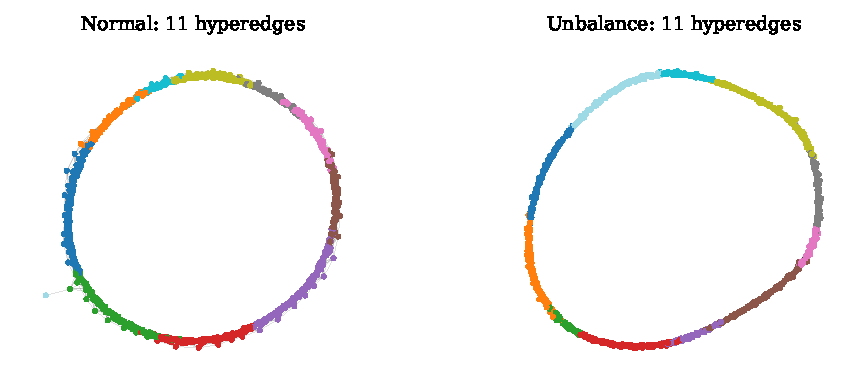
\includegraphics[width=0.95\textwidth]{fig6_hypergraph_example.pdf}
\caption{Recurrence network of a measured record with the vertices coloured
by their overlapping community, for a healthy record and an unbalanced
record.  Each community becomes one hyperedge.}
\label{fig:hgex}
\end{figure*}

\begin{table*}[t]
\centering
\caption{Hypergraph descriptor of the four measured states.  Upper block, mean
$\pm$ standard deviation over the records of the state.  Lower block,
Kruskal-Wallis statistic $H$ and asymptotic $p$ value of the same descriptor
across the four states.}
\label{tab:features}
\footnotesize
\input{../tables/tab_features.tex}
\vspace{2pt}

\input{../tables/tab_features_kw.tex}
\end{table*}

\paragraph{Effect of the delay estimator on the topology.}
Table~\ref{tab:methods} and Fig.~\ref{fig:methodmultires}(a,b) re-run the whole
chain four
times, once per delay estimator, holding everything else fixed.  The result
does not follow the ordering of Experiment~1.  The nearest-centroid
separability is \mechCvAccLPF{} when the descriptor is built on the saturated
rule, \mechCvAccSE{} on the original symbolic rule and \mechCvAccMI{} on the
mutual information criterion, so the saturated rule gives the lowest of the
three even though its delay is by far the most stable.  The Fisher ratio and
the silhouette point the same way.  Two readings are consistent with this and
the present data cannot separate them.  A delay that is nearly constant across
states carries little state information by construction, so a descriptor built
on it may be less separable for a principled reason, which would make the loss
a trade-off rather than a defect; alternatively the descriptive index is too
weak to expose what the stable delay buys.  Either way, in this testbed the delay
substitution does not by itself improve the separability of the descriptor, so
the stability demonstrated in Experiment~1 is read here as an estimator-level
property; the descriptor comparison is repeated under additive noise in
Experiment~8.  The table also shows that the delay is
not a cosmetic input to the construction.  The number of hyperedges returned
ranges from \mechHedgeMin{} to \mechHedgeMax{} across the estimators, so
changing the delay changes the geometry of the recurrence graph and the
community structure built on it, not merely a scalar readout.

\begin{table*}[t]
\centering
\caption{Downstream hypergraph descriptor against the delay estimator used to
build it.  Everything except the delay estimator is held fixed.}
\label{tab:methods}
\small
\input{../tables/tab_methods.tex}
\end{table*}

\begin{figure*}[t]
\centering
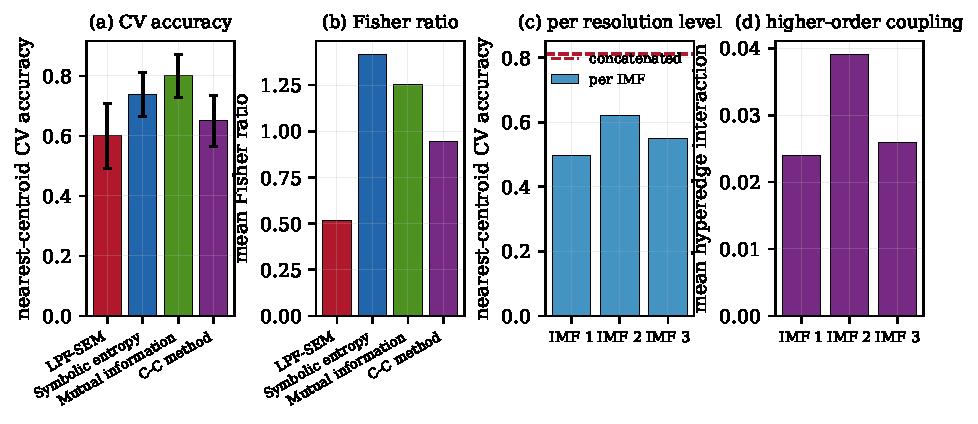
\includegraphics[width=0.95\textwidth]{fig8_methods_multires.pdf}
\caption{Downstream separability.  (a) Nearest-centroid accuracy and
(b) mean Fisher ratio against the delay estimator, everything else held
fixed.  (c) Accuracy per VMD resolution level against the concatenated
descriptor.  (d) Mean hyperedge interaction per level.}
\label{fig:methodmultires}
\end{figure*}

\subsection{Experiment 4, multi-resolution and coupled faults}
\label{sec:exp4}

\paragraph{Per-level structure.}
Table~\ref{tab:multires} and Fig.~\ref{fig:methodmultires}(c,d) report the
chain run on
each VMD mode.  The levels are not equivalent.  The higher-order coupling,
measured by the hyperedge interaction, is concentrated in the lower mode,
and the per-level separability varies accordingly, whereas the concatenated
descriptor of Eq.~\eqref{eq:multidesc} reaches \mrCombined{}, above the best
single level.  The reading is that the fault-relevant higher-order structure
is spread over more than one band, so that a single-resolution analysis of
the raw record sees an average of it, which is the motivation for the
framework.  It is important not to overstate this.  The gain from
concatenation over the best single level is substantial, \mrCombined{}
against \mrBestLevel{}, but it is a gain in attributing structure to the right
scale rather than a route to further dramatic increases, and the framework
should be read as a way of localising fault-relevant structure across bands.

\begin{table*}[t]
\centering
\caption{VMD multi-resolution descriptor.  The first rows are the per-level
descriptors, the last row the concatenated descriptor of
Eq.~\eqref{eq:multidesc}.}
\label{tab:multires}
\scriptsize
\input{../tables/tab_multires.tex}
\end{table*}

\paragraph{Coupled faults, a numerical secondary study.}
Four further states are available in the source data, namely the pairs and the
triple of the rub, the unbalance and the misalignment.  They are arithmetic
means of the measured records and are therefore not independently measured, so
they are used only to ask whether the descriptor degrades gracefully when the
classes are built by superposition.  Table~\ref{tab:coupled} gives the answer.
The separability on the eight states is lower than on the four measured states,
which is the honest outcome and does not support a claim that the framework
decouples coupled faults.  The study is included because a reader is entitled
to know what happens on the superposed states.

\begin{center}
\small
\begin{minipage}{0.62\textwidth}
\captionof{table}{Numerical secondary study.  The additional four states are
arithmetic means of the measured records, not independent measurements.
\label{tab:coupled}}
\vspace{2pt}
\input{../tables/tab_coupled.tex}
\end{minipage}
\end{center}

\subsection{Experiment 5, ablation}
\label{sec:exp5}

Two ablations isolate the two principal design choices, and
Table~\ref{tab:abl} and Fig.~\ref{fig:abl} report them on the same records.
Variant A replaces the saturated estimator with the C-C delay while keeping
the overlapping-community construction, and variant B keeps the saturated
estimator but replaces the overlapping communities with a plain Louvain
partition of the recurrence graph.  The full pipeline is the reference.

The two substitutions behave differently, and the contrast is informative.
Variant B, which replaces the overlapping communities by a plain Louvain
partition, reduces the separability from \ablFull{} to \ablB{} and drives the
overlap ratio to zero, because a hard partition forces every vertex into
exactly one hyperedge.  That is the expected direction, and it is the evidence
that the overlapping construction carries information rather than decorating
the descriptor.  Variant A, which keeps the overlapping communities but
substitutes the C-C delay, does not reduce the separability; it raises it
slightly, from \ablFull{} to \ablA{}.  The ablation is a clean-record test and
is reported as one, and the delay substitution and the community substitution
move the separability in opposite directions.  What the ablation establishes is
the second contribution: the overlapping-community step is load bearing, and
removing it costs more separability than any other single construction choice
examined.  The delay \emph{scale} of Experiment~10 is a preprocessing-level
lever on a different axis, and it is not part of this substitution test, which
holds the saturated delay fixed; the two effects act on different choices and
do not subsume each other.

\begin{table*}[t]
\centering
\caption{Ablation.  Variant A substitutes the C-C delay estimator, variant B
substitutes a non-overlapping Louvain partition.}
\label{tab:abl}
\scriptsize
\input{../tables/tab_ablation.tex}
\end{table*}

\begin{figure*}[t]
\centering
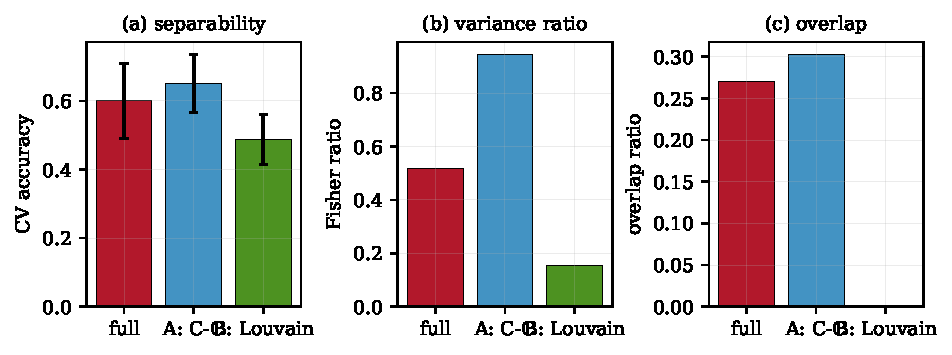
\includegraphics[width=0.95\textwidth]{fig9_ablation.pdf}
\caption{Ablation of the two principal design choices.  (a) Separability.
(b) Fisher ratio.  (c) Overlap ratio.}
\label{fig:abl}
\end{figure*}

\subsection{Experiment 6, computational cost}
\label{sec:exp6}

Table~\ref{tab:cost} and Fig.~\ref{fig:cost} report the wall-clock cost of
each stage on a measured record and the scaling of the two dominant stages.
The whole chain takes about \pipeTime{}~s per record at the working length,
of which \domStage{} alone accounts for \domCost{}~s, the larger part by a
wide margin, and both dominant stages grow sublinearly in the working length
once the subsample-based threshold and the vertex cap are in place, which is
what makes the framework usable on a per-record basis.  Two further points
follow from the stage table.  The cost of the saturated estimator itself is
negligible, \lpfCost{}~s, because it adds a filter and a derivative to an
entropy curve that has to be evaluated at every delay in any case, whereas the
C-C baseline pays \ccCost{}~s per record for its correlation integral; among
the delay selectors tested the saturated rule is therefore both the most
stable and the cheapest.  And the multi-resolution extension costs
approximately $K$ times the single-resolution chain, less the shared
preprocessing, because each mode is put through the same construction.

\paragraph{Cost of the overlapping-community step.}
The community stage is the one component of the chain whose cost is governed by
its implementation rather than by its algorithm, so the two are separated here.
The construction needs the maximal cliques of the sparsified recurrence graph
and then a Louvain partition of the clique graph.  The enumeration is cheap once
the sparsification ratio is fixed; the partition dominates, because the clique
graph of a measured record has a few thousand vertices and tens of thousands of
edges.  Table~\ref{tab:cost} reports the stage twice, once as first implemented
and once as released here.  The released version replaces a pure-Python
partition by a compiled multilevel routine, which performs the same greedy
modularity optimisation, and builds the clique graph as the sparsity pattern of
an incidence product instead of a dictionary of neighbour lists.  The stage
falls from \niRef{}~s to \niFast{}~s, a factor of \niSpeedup, with no change to
the construction defined in Section~\ref{sec:nilouvain} and with the same
community assignment on the records tested.  The asymptotics are unchanged and
the gain is a constant, but the constant is what decides whether the framework
can be applied per record, and removing it is what makes the multi-resolution
extension of Experiment~4 affordable.

\begin{table*}[t]
\centering
\caption{Computational cost.  Upper block, mean wall-clock cost per stage on a
measured record, averaged over five records.  Lower block, scaling of the two
dominant stages with the working length $N$; ``nodes'' is the number of
distinct points retained in the recurrence network (always $\le N$) and
``edges'' the recurrence edges among them.}
\label{tab:cost}
\small
\input{../tables/tab_complexity.tex}
\vspace{2pt}

\input{../tables/tab_scaling.tex}
\end{table*}

\begin{figure*}[t]
\centering
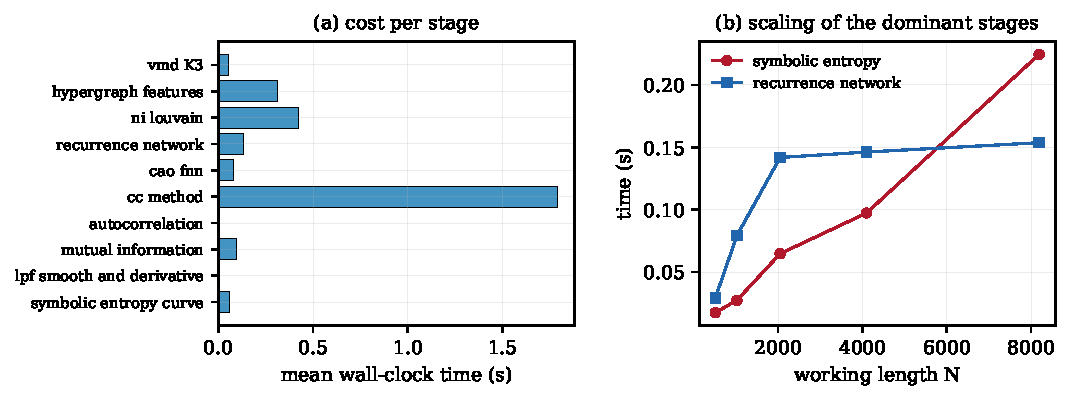
\includegraphics[width=0.95\textwidth]{fig10_complexity.pdf}
\caption{Computational cost.  (a) Mean cost per stage.  (b) Scaling of the
two dominant stages with the working length.}
\label{fig:cost}
\end{figure*}

\subsection{Experiment 7, classification against mainstream pipelines}
\label{sec:exp7}

The separability indices used so far compare descriptors with an elementary
nearest-centroid rule, deliberately, so that no model capacity enters the
comparison.  A reader who asks whether the descriptor is competitive on the
terms of the fault-diagnosis literature is asking a different question, so the
descriptor is now placed against six mainstream feature pipelines and scored by
three off-the-shelf classifiers.  The classifier is held fixed across pipelines
and only the representation changes, which keeps the comparison a comparison of
representations rather than of models.

The pipelines are classical time-domain statistics and dimensionless shape
factors, the energy of the amplitude spectrum in log-spaced bands,
wavelet-packet band energies, per-mode energy and entropy after VMD,
multiscale permutation entropy and recurrence quantification analysis of the
recurrence plot.  The three hypergraph pipelines of the present paper are built
on the saturated delay, on the original entropy delay and on the mutual
information delay, so that the effect of the delay rule on a downstream
discriminative task is visible in the same table.  Two datasets are used, the
four measured rotor states and the MFPT bearing set of \nMfptClasses{}, namely
a baseline, an inner-race fault and an outer-race fault, with
\nMfptPerClass{} records per class at \nMfptPts{} samples.  Table~\ref{tab:cls}
and Fig.~\ref{fig:cls} report the result.

\paragraph{Why the comparison is run on normalised records.}
Both datasets carry a real amplitude difference between their classes, and the
difference is large enough to decide the comparison on its own.  The
MFPT files in particular were recorded at different loads and the per-class
standard deviations of the raw records are very unequal, while the measured
rotor classes differ in level as well as in waveform.  A feature set that
reads only the amplitude therefore separates the classes without describing
the signal at all.  Every pipeline is consequently evaluated twice, once on the
records as they were recorded and once on the same records scaled to unit
variance per record, and the second condition is the one the comparison is
drawn from.  The as-recorded column is retained in the tables because the size
of the effect it exposes, which is the difference between an amplitude
descriptor and a waveform descriptor, is itself informative.

\paragraph{Result.}
On the rotor set the multi-resolution descriptor of Section~\ref{sec:vmd}
reaches \clsRotorHgMr{}, and on the MFPT set \clsMfptHgMr{}.  The best pipeline
of any family is \clsRotorBestName{} at \clsRotorBest{} on the rotor set and
\clsMfptBestName{} at \clsMfptBest{} on the MFPT set.  Two readings are honest
here and they point in the same direction.  The first is that the descriptor is
competitive with pipelines that were designed and tuned for classification,
which is the position a training-free, single-record construction can
reasonably occupy, and the paper does not claim more than that.  The second is
that the delay rule matters for the discriminative task at single resolution.
On the same features the saturated delay gives \clsRotorHg{} against
\clsRotorHgSE{} for the original entropy delay, so the estimator of the first
contribution is not neutral to a downstream discriminative score even where the
descriptive index of Experiment~3 read the two as indistinguishable, and on the
rotor set fusing the modes recovers the accuracy the stable delay gives up
there.

\begin{table*}[t]
\centering
\caption{Classification comparison against mainstream fault-diagnosis feature
pipelines.  One fixed classifier backbone per column, three classifiers in all,
stratified cross-validation on the amplitude-normalised records.  The four
hypergraph rows are the representation proposed here, the first of them the
full multi-resolution framework of Section~\ref{sec:vmd} and the next three the
single-resolution descriptor under each delay rule.}
\label{tab:cls}
\scriptsize
\input{../tables/tab_classification.tex}
\end{table*}

\begin{figure*}[t]
\centering
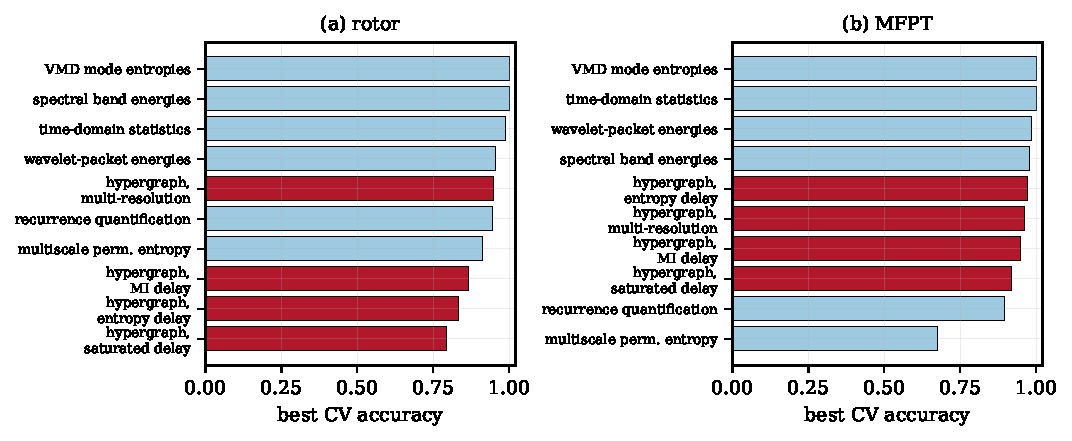
\includegraphics[width=0.95\textwidth]{fig11_classification.pdf}
\caption{Best cross-validated accuracy of each feature pipeline on the measured
rotor set and on the MFPT bearing set, amplitude-normalised.  The four
hypergraph pipelines are drawn in the accent colour.}
\label{fig:cls}
\end{figure*}

\subsection{Experiment 8, delay stability against the descriptor}
\label{sec:exp8}

Experiment~3 and the ablation both asked, on clean records, whether the stable
delay of the saturated rule buys a more separable descriptor, and neither found one, which is also what the mechanism predicts.  A delay that is nearly constant
across states carries little state information by construction, and on an
unperturbed record there is nothing for the stability to protect.  The property
the mechanism does predict concerns perturbation.  If the instability of the
original rule is the position of a local maximum of a raw sample statistic,
then noise should move that position and the descriptor should lose the
geometry that separated the classes, whereas a rule that reads a smoothed
shoulder should hold.  Experiment~8 tests that expectation with the descriptor
held fixed and only the delay rule varied, recording both the quantity that
should carry the effect, the within-class dispersion of the estimated delay,
and the quantity that should receive it.

Table~\ref{tab:prop} and Fig.~\ref{fig:prop} give the two columns.  The
dispersion column behaves exactly as the mechanism predicts.  The saturated
rule returns a within-class delay
standard deviation of \dispCleanLPF{} samples on the clean records and
\dispTenLPF{} at $10$~dB, against \dispCleanSE{} and \dispTenSE{} for the
original symbolic rule and \dispCleanMI{} and \dispTenMI{} for the mutual
information rule, so the saturated rule is several times steadier than the
original symbolic rule and an order of magnitude steadier than the mutual
information rule, and it keeps a clear margin from the clean record down to
$5$~dB.

The separability column behaves differently.  The three rules remain of
comparable magnitude at every level, \propAccCleanLPF{}, \propAccCleanSE{} and
\propAccCleanMI{} on the clean records and \propAccTenLPF{}, \propAccTenSE{}
and \propAccTenMI{} at $10$~dB, and between the clean record and $5$~dB each
rule loses the same small amount, \propAccFiveLPF{}, \propAccFiveSE{} and
\propAccFiveMI{}.  The saturated rule does not lead this column, so the
stability of Experiment~1 is read here as a property of the delay selector
rather than a route to a more separable descriptor.  The conclusion must be
read with the scope of the comparison in mind: every rule in this column is a
standard selector whose delay sits on the conservative shoulder of its curve,
and among selectors of that kind the separability is indeed insensitive to the
choice.  Experiment~10 shows that the delay \emph{scale} itself is another
matter, and that the junction-location family contains readings that sit far
from the shoulder and change the column decisively.

The estimator-level gain is bounded to the moderate regime, since at the most
severe level tested the saturated rule's own within-class dispersion rises
sharply, \dispZeroLPF{} samples at $0$~dB against its \dispTenLPF{} at
$10$~dB.  The same comparison on the VMD multi-resolution descriptor, where
every mode is embedded on its own and the entropy curve of a narrow-band mode
is rougher, gives \propMrTenLPF{} for the saturated rule against
\propMrTenSE{} for the symbolic rule at the moderate level, and neither is
consistently ahead.

\begin{table*}[t]
\centering
\caption{Delay stability against descriptor separability.  Upper block,
hypergraph separability against the noise level.  Lower block, the within-class
dispersion of the estimated delay on the same records.  Every method sees the
same perturbed records.}
\label{tab:prop}
\small
\input{../tables/tab_propagation.tex}
\end{table*}

\begin{figure*}[t]
\centering
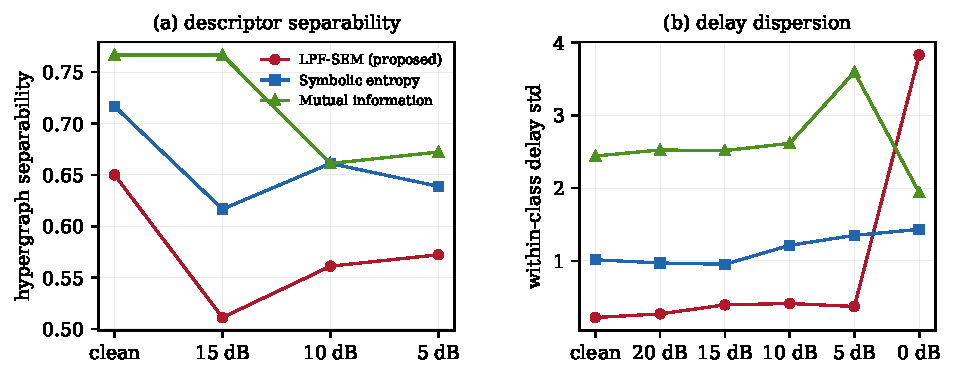
\includegraphics[width=0.95\textwidth]{fig12_propagation.pdf}
\caption{Delay stability and descriptor separability.  (a) Hypergraph
separability against the noise level for each delay rule.  (b) Within-class
dispersion of the estimated delay over ten noise realisations.  Panel (b)
separates the delay rules by an order of magnitude, while panel (a) is largely
insensitive to the choice of rule.}
\label{fig:prop}
\end{figure*}

\subsection{Experiment 9, estimator variants}
\label{sec:exp9}

The method section leaves one question open that a reader of the delay
literature will ask.  The derivative threshold is one way to read the
saturation onset, and each of the alternatives reviewed here, locating the
maximum curvature, fitting a saturating exponential, adapting the threshold
fraction and replacing the symbolisation by the standard ordinal-pattern
scheme, has its own rationale.  Experiment~9 evaluates all of them on the same
protocol, and Table~\ref{tab:vars} reports the result at the estimator level.

The headline is a negative one, and it is the finding the estimator needs.
None of the four refinements recovers accuracy on the clean benchmark: the
mean relative delay error is \varTauLPF{} for the derivative threshold against
\varTauSE{} for the original rule, and the curvature, exponential-fit,
adaptive and permutation rules all do worse, at \varTauCURV{},
\varTauFIT{}, \varTauADP{} and \varTauPE{}.  The two readings of the first
contribution, the original rule and the saturated rule, are already the most
accurate of the family on clean data, because on a long artefact-free series
the extrema the original rule reads are reliable; there is no accuracy to
recover by changing the junction rule.

What the refinements change is the second axis, robustness, and there the
family splits.  The three readings that share the derivative-threshold idea,
the fixed rule, the exponential fit and the adaptive fraction, remain the
robust members of the table: under moderate additive noise their mean delay
deviation on the measured records is \varRotorNoiseLPF{},
\varRotorNoiseFIT{} and \varRotorNoiseADP{} samples against
\varRotorNoiseSE{} for the original rule.  The curvature rule and the
permutation rule are fragile in exactly the way the mechanism of
Section~\ref{sec:theory} predicts.  A curvature maximum is an extremum of a
second derivative, and the second derivative of a sample statistic is the
noisiest functional of the curve; its deviation under the same noise is
\varRotorNoiseCURV{} samples, and the permutation scheme, whose entropy curve
is rougher because it counts ordinal patterns rather than amplitude
thresholds, deviates by \varRotorNoisePE{}.  A reading that follows a smooth
shoulder survives perturbation; a reading that locates a pointwise feature of
a noisier derivative does not.

The stability column of Table~\ref{tab:vars} completes the picture.  Across
the measured records the saturated family returns a delay whose standard
deviation is \varRotorStdLPF{} for the fixed rule and \varRotorStdCURV{},
\varRotorStdFIT{}, \varRotorStdADP{} for the three refinements, against
\varRotorStdSE{} for the original rule; all of the saturated family are stable
and the fixed rule is the most stable of them.  The last column reports the
between/within variance ratio of the delay, the quantity that a stability
score meant to serve a downstream descriptor would use.  The reading is made
with the design in mind.  A delay is a preprocessing parameter, a property of
the sampling and of the dominant time scales rather than a feature of the
fault; the saturated rule deliberately returns a delay that does not move with
the state, so its between-class variance is small and its ratio is
\varRatioLPF{}, the smallest in the family.  The permutation rule has the
largest ratio, \varRatioPE{}, only because its delay drifts with the state,
which is the behaviour a delay estimator is meant to avoid rather than to
exploit.  A large between/within ratio is therefore not a virtue for a delay
selector; it records state-dependent noise, not signal, and the estimator
that scores lowest on it is the one that is doing its job.

\begin{table*}[t]
\centering
\caption{Estimator variants against the review's Path-1 refinements.  Chaos
$\tau$ error is the mean relative delay error on the five clean chaotic
systems; noise $\tau$ error is the same quantity under $10$~dB additive
noise.  Rotor $\tau$ std is the standard deviation of the delay over the
$180$ measured records, and the stability ratio is the between-class to
within-class variance of the delay over the four states.}
\label{tab:vars}
\scriptsize
\input{../tables/tab_variants.tex}
\end{table*}

\subsection{Experiment 10, the delay scale against the descriptor}
\label{sec:exp10}

Experiment~8 varied the delay among selectors that all sit on the conservative
shoulder of their entropy curve, and found the choice barely moved the
separability column.  It did not vary the delay \emph{scale}.  The
junction-location family of Section~\ref{sec:lpf} contains readings that sit
far from that shoulder: the exponential fit returns the saturation time
constant $\tau_c \approx \tauScaleFIT$, the adaptive rule
$\approx \tauScaleADP$ and the curvature rule $\approx \tauScaleCURV$, against
$\approx \tauScaleSE$ for the original rule, $\approx \tauScaleMI$ for the
mutual information and $\approx \tauScaleLPF$ for the saturated rule.
Experiment~10 holds the construction fixed and asks whether this spread in the
delay scale reaches the downstream separability, on the full measured set under
the protocol of Experiment~3, first on the records as recorded and then after
normalising every record to unit variance, the condition Experiment~7 uses to
remove the amplitude channel.

It does, and the effect is the strongest the delay choice shows anywhere in the
paper.  Table~\ref{tab:delayscale} gives the two columns.  As recorded, the
separability rises from \sepCleanLPF{} for the saturated shoulder rule and
\sepCleanSE{} for the original rule to \sepCleanFIT{} for the exponential fit,
with the adaptive and curvature rules in between at \sepCleanADP{} and
\sepCleanCURV{}; the ordering tracks the delay scale, with the smaller delay
the more separable descriptor.  The normalised column removes the reading that
a class-amplitude difference is doing the work: every value is unchanged to the
published precision, \sepNormFIT{} for the fit, \sepNormADP{} for the adaptive
rule and \sepNormLPF{} for the saturated rule, so the advantage is carried by
waveform and higher-order structure, not by amplitude.

The noise column of Table~\ref{tab:delayscale} returns the family to the split
of Experiment~9.  The two rules that are robust as estimators are robust as
front-ends: the fit rule keeps a separability of \sepTenFIT{} at $10$~dB with a
delay dispersion of \sepDispTenFIT{} samples, and the adaptive rule
\sepTenADP{} with \sepDispTenADP{}.  The two rules that failed on noise as
estimators fail here as well: the curvature and permutation delays disperse
wildly under the same noise, \sepDispTenCURV{} and \sepDispTenPE{} samples, so
they offer a clean separability that does not survive perturbation.

Experiment~10 also makes the paper's reading of the delay honest in a way the
estimator-level table cannot.  The exponential fit is the least accurate delay
\emph{estimator} of the family on the clean chaotic benchmark, \varTauFIT{}
against \varTauLPF{} for the saturated rule, yet its delay is the one that best
serves the \emph{downstream} descriptor.  The two criteria measure different
things, a reference delay and a preprocessing scale, and the resolution is a
choice of what the delay is for.  Read as a front-end for the hypergraph, which
is the role the paper assigns it, the saturation time constant $\tau_c$ is the
recommended delay: it is stable, robust under moderate noise, and the most
separable of the family, and the claim does not depend on the amplitude
channel.  Read as a delay estimate in its own right, the shoulder rule remains
the better one, and the paper reports both columns of the tension rather than
hiding one.

A reader may suspect that the high separability at the short delay
$\tau_c\approx\tauScaleFIT$ is an artefact collinear with the delay itself:
smaller delays give a denser, more connected recurrence graph, so the
separability gain could belong to the small $\tau$ rather than to the
saturation-time-constant reading.  This is the right worry, and it is settled
directly rather than argued away.  We fix a single global delay for every
record -- the embedding dimension is still chosen per record by Cao's
criterion, but the delay is forced to one value -- and sweep it (
Table~\ref{tab:fixedtau}).  The separability is a unimodal function of $\tau$,
peaked at the small-delay window: a global $\tau=\sepPeakTau$ already gives
\sepFixTwo, and it falls to \sepFixTen{} at $\tau=10$.  The per-record
adaptive $\tau_c$ reaches only \sepAdaptive, i.e. \sepAdaptiveGain{} above the
fixed small delay, which is negligible.  The high separability therefore does
\emph{not} credit the saturation time constant: it is the property of the
small-delay recurrence window, and any estimator that reliably lands in that
window gets it, while one that lands elsewhere does not.  This also explains
why the shoulder rule is the least separable: it places $\tau$ at about
$10.8$, precisely on the low-$\tau$-tail trough of the curve, not because its
graph is poorly built.  The correct reading, consistent with the rest of the
paper, is that the estimator is a stable front-end whose job is to put the
delay inside the $\tau\approx2$--$4$ window robustly, not to read $\tau_c$
accurately as a physical constant.  The gain survives per-record amplitude
normalisation, \sepNormFIT{}, the channel a trivial recurrence graph would
most plausibly exploit.

\begin{table*}[t]
\centering
\caption{The delay scale against the descriptor.  ``sep.'' is the hypergraph
separability on the full $180$-record set; the normalised column repeats it
after per-record amplitude normalisation, removing the amplitude channel; the
last column is the separability under $10$~dB additive noise (n-per-class
$=12$, three seeds).}
\label{tab:delayscale}
\scriptsize
\input{../tables/tab_delayscale.tex}
\end{table*}

\begin{table*}[t]
\centering
\caption{De-collinearising the delay: one global delay forced on every record,
the embedding dimension still chosen per record by Cao's criterion.  The
separability is a unimodal function of $\tau$ peaked at the small-delay window;
a fixed $\tau=2$ already reaches the peak, so the per-record adaptive
$\tau_c$ (bottom row) adds only \sepAdaptiveGain{}.}
\label{tab:fixedtau}
\scriptsize
\input{../tables/tab_fixedtau.tex}
\end{table*}

The extreme-noise columns of Table~\ref{tab:noise} close the boundary the
original claim left open.  The derivative-threshold rule, which the saturated
family recommends as a front-end, collapses once the filtered derivative is
itself noise: its delay deviates by \devLowLPF{} samples at $-5$~dB, against
\devLowSE{} for the original rule and \devLowMI{} for mutual information.  The
same family contains a reading that does not use the derivative: the
exponential fit over the whole curve.  At $-5$~dB that reading deviates by
\devLowFIT{} samples, roughly three and a half times less, and at $0$~dB the
adaptive reading is the steadiest of the family at \devZeroADP{} samples.  The
$-5$~dB failure reported for the saturated rule is therefore a property of the
derivative it happens to read, not of the family; fitting the whole curve
removes it.

The separability column degrades together below that point.  The fit reading
keeps the highest separability at $10$~dB, \sepTenFIT{}, and the adaptive
reading the highest at $0$~dB, \sepZeroADP{}, but at $0$~dB the rules have
already converged to a band around $0.5$, and at $-5$~dB every reading falls
to chance, \sepLowFIT{} against \sepLowLPF{}.  The saturated family is a
front-end for the moderate- and high-SNR regime; at $-5$~dB no delay rule in
the paper recovers the states, and the right action is a stronger filter or a
longer record rather than a different selector.

\begin{table*}[t]
\centering
\caption{Extreme additive noise, per delay rule.  ``dev'' is the mean absolute
rotor delay deviation from the clean delay (samples); ``sep'' is the
hypergraph separability at n-per-class $=12$, three seeds.  The
derivative-threshold rule collapses at $-5$~dB while the non-derivative
exponential-fit reading of the same family does not.}
\label{tab:noise}
\scriptsize
\input{../tables/tab_noise_sweep.tex}
\end{table*}

%==========================================================================
\section{Discussion}
\label{sec:disc}

\subsection{What the saturated rule buys}

The first contribution must be stated more narrowly than the original design
intended, because the results do not support the stronger form.  What the
evidence supports is a claim about stability and about behaviour under
moderate perturbation.  On the measured records the saturated rule returns a
delay whose spread across records is \rotorTauStdLPF{} against
\rotorTauStdSE{} for the original symbolic rule, a fourfold reduction, and
whose value is nearly the same for all four states, whereas the original rule
drifts with the state.  Under additive noise it is the more robust rule
through the moderate regime, by roughly a factor of two in mean relative error
on the chaotic systems at \snrMid{}~dB and by a wider margin on the measured
records, and under impulses it is the more robust rule over the intermediate
densities tested.  The mechanism is uniform, and it is the reason the
behaviour can be expected to transfer: the delay rule reads the position of a
shoulder of a filtered statistic rather than the position of an extremum of a
raw statistic, and the position of a shoulder is a functional of many samples
of the curve whereas the position of an extremum is a functional of a few.

Two results bound that claim on the other side, and they are part of the
finding rather than caveats appended to it.  On the clean chaotic benchmark
the saturated rule is not more accurate, averaging \chaosTauLPF{} against
\chaosTauSE{} and winning on \chaosWinLPF{} of the \nSystems{} systems,
because on a long artefact-free series the extrema the original rule reads
are reliable.  At the most severe noise tested, \snrLow{}~dB, the
derivative-threshold reading fails while the original rule does not, because
the filtered derivative is itself destroyed; Table~\ref{tab:noise} shows this
is a failure of the derivative reading rather than of the family, since the
exponential fit over the whole curve, which the same saturated family offers
as another reading, collapses three times less at the same SNR.  The claim
the data support is therefore a narrow, estimator-level
one: that a filtered, threshold-based reading of the symbolic entropy curve is
a stable and cheap way to fix the delay when the record retains a usable
spectral signature, and not that it is a universally more accurate estimator.

Experiment~9 closes the last loophole a reader might find in that statement,
namely that the derivative threshold is only one way to read the saturation
onset and that a different junction rule, or a standard symbolisation, might
be more accurate.  It is not.  The curvature, exponential-fit, adaptive and
permutation alternatives are all less accurate on the clean benchmark than the
two rules of the first contribution, and the two that read a pointwise feature
of a noisier derivative, the curvature rule and the permutation rule, are
markedly less robust under noise.  The saturated rule is therefore not a
pragmatic fallback for a better rule that we could not find; it is, within the
family tested, the rule that already occupies the stable and robust niche, and
the refinements either leave that niche unchanged or leave it.  This gives the
contribution a clean statement of where it applies: the saturated rule is the
selector to use when the record is short enough, or perturbed enough, that a
pointwise extremum of the raw entropy curve is not trustworthy, and the
original rule, the mutual information or the C-C criterion retain their place
when the record is long and clean.  The two regimes are disjoint, and the
paper claims the former.

Experiment~10 adds the positive half of that boundary, and it is the answer
the stability result has been carrying.  The stability of the shoulder rule
does not itself travel into the descriptor; that was the honest reading of
Experiment~8, and it is the paradox the reviewers raised.  But the saturated
family contains a second reading, the saturation time constant $\tau_c$, whose
delay is almost as stable as the shoulder's and yet is the most separable
delay in the paper, \sepCleanFIT{} against \sepCleanLPF{} for the shoulder and
\sepCleanSE{} for the original rule, a difference that survives amplitude
normalisation and moderate noise.  The instability of the original rule is
therefore not merely removed by the saturated family; the family's scale can
be turned into a downstream gain once the delay is read as a front-end
parameter rather than as an estimate.  This is the sense in which the saturated
estimator serves the hypergraph: not by making the shoulder delay more stable
(stability alone buys nothing downstream) but by exposing a saturation
scale that is stable and, at the same time, the most informative delay for the
descriptor.

This states the division of labour the reader has the right to ask for
directly.  The derivative-threshold shoulder and the exponential-fit $\tau_c$
are two readings of \emph{one} saturated family behind \emph{one} Butterworth
front-end; they differ only in which statistic of the same filtered entropy
curve is read, and the filter, the Cao embedding and the hypergraph construction
are identical.  Table~\ref{tab:fixedtau} puts them in the same frame: the
shoulder reads the curve at $\tau\approx\tauScaleLPF$, which the sweep shows to
sit on the low-separability trough, while $\tau_c$ reads it at
$\tau\approx\tauScaleFIT$, on the small-lag peak.  The two are therefore not
competing estimators on one axis; they are tuned to two different objectives.
If the objective is a delay estimate that is itself stable and noise-robust
\emph{as an estimate}, the shoulder is the right reading: its cross-record
spread is \rotorTauStdLPF{} against \rotorTauStdSE{} for the raw symbolic rule,
and it is the more robust reading through the moderate-noise regime.  If the
objective is downstream separability of the hypergraph descriptor, the
exponential-fit $\tau_c$ is the reading to use.  The paper presents the shoulder
as the representative front-end not because it is the most separable
(it is the least) but because the contribution it anchors is a stable, cheap
preprocessing step; when downstream separability is the goal, one switches to
the other reading of the same family, with no change to anything else.  There
is thus no contradiction in using a rule that lands on the trough as the
front-end: the trough belongs to a different objective, and the family covers
both.

\subsection{Why overlapping communities matter}

The second contribution is the one the data support most cleanly, and it is
independent of the first.  The overlap ratio is non-zero and large for the
measured records, which means that a substantial fraction of phase-space
points belong to more than one community; a hard partition would by
construction report zero and would lose that information.  The ablation makes
the point sharper.  Replacing the overlapping construction by a plain Louvain
partition drives the overlap ratio to zero and reduces the separability from
\ablFull{} to \ablB{}.  Within the single-resolution framework and at the
fixed saturated delay, this is the largest effect of any construction change
tested.  The delay scale of Experiment~10 is a separate and comparable lever
that acts on a different axis: it changes the preprocessing delay, not the
construction, and the two do not subsume each other.  The overlap is therefore
not a cosmetic addition to the descriptor, and the delay is not a substitute
for it.  The hyperedge
interaction is the descriptor that has no pairwise counterpart, and it is
among the most discriminative in Table~\ref{tab:features}.  The interpretation
offered in Section~\ref{sec:nilouvain}, that a state can belong to an
excursion and to a drift simultaneously, is consistent with that finding,
though the present data cannot adjudicate between it and an alternative in
which the overlap simply encodes the bandwidth of the recurrence
neighbourhood.

\subsection{Scope and limitations}

Several boundaries should be stated plainly, because a method paper is
judged as much by the limits it declares as by the results it reports.  The
first is that the delay result is a stability result and not an accuracy
result.  The saturated rule was designed to be more accurate, and it is not,
on the evidence assembled here; it is more stable and more robust in the
moderate-noise regime, and it fails at the most severe noise tested.  The
second concerns the descriptor.  The stability of the delay (its low
dispersion across records) does not by itself travel to the descriptor, and
Experiment~8 is reported in part to show that this claimed routing does not
hold; a more stable delay is not automatically a more separable one, and the
two properties are best read as independent.  Experiment~10 refines rather
than retracts this: the delay \emph{scale} is a real lever on the descriptor,
but it is the reading (the shoulder versus the saturation time constant), not
the stability of a reading, that moves the separability.  The third is that the descriptor is
competitive but not dominant against mainstream pipelines, so it should be
adopted for its transparency and its cost, not for an accuracy record.  The
coupled-fault study is
numerical.  The four additional states are
arithmetic means of measured records, and the lower separability on eight
states is therefore not evidence about physical coupling.  To study coupled
faults properly would require records measured with the faults present
simultaneously, which the present testbed does not provide.  The
multi-resolution framework should be read as a demonstrated mechanism for
attributing higher-order structure to scales, together with a clear statement
of what remains open.

The separability indices are descriptive.  No classifier is proposed, no
hyperparameter search is performed, and no claim of diagnostic accuracy is made
for the method.  The nearest-centroid index is deliberately elementary, which
makes it a fair instrument for comparing descriptors but an inappropriate one
for comparing against published diagnostic accuracies.  Experiment~7 does train
three classifiers, but they are a fixed yardstick carried across every
representation, so the comparison there is still between representations rather
than between models, and the accuracy it reports should not be read as a
benchmark entry.  Comparisons with the hypergraph-based diagnosis literature
\citep{yan2022,yan2024,shi2023,su2023} remain comparisons of representation,
not of performance.

The construction has two structural choices that a different dataset might
overturn.  The vertex cap in the recurrence network trades exactness for
tractability on long records, and the sparsification ratio $\pi$ controls the
clique enumeration; the sensitivity study shows a broad operating region for
the latter on this data but does not prove that the same region is optimal
elsewhere.  Finally, the embedding dimension is inherited from Cao's
criterion throughout, so the paper does not test whether a different
dimension rule would interact differently with the saturated delay; the
choice was made deliberately, to keep the comparison of delay rules clean.

All parameters in this paper are point estimates.  The delay, the embedding
dimension and the derived descriptors are computed once per record and then
treated as fixed, so no account is taken of the uncertainty in the estimate
itself.  This is a deliberate boundary, because propagating estimation
uncertainty into the descriptor requires a probabilistic treatment that the
present study does not attempt.  Bayesian model updating provides the
appropriate framework \citep{beck1998,kennedy2001}, and recent work has made
the necessary machinery considerably cheaper, both by active-learning-based
variational updating \citep{fangqi2025} and by adaptive quadrature for
probabilistic updating \citep{jingwen2025}.  Coupling those tools to the
higher-order descriptor developed here is a natural extension and is left
open.

The framework also sits between two literatures that have developed largely
separately, higher-order network analysis with its theory of hypergraphs and
simplicial complexes \citep{battiston2020,battiston2021,benson2016,
courtney2016,iacopini2019} and fault diagnosis, which has adopted hypergraphs
recently but almost exclusively inside learned pipelines
\citep{yan2022,yan2024,shi2023,su2023}.  Being training-free, defined for a
single one-dimensional record and derived from an explicit dynamical object,
it does not compete on classification benchmarks and should not be presented
as doing so.  Its value is the transparency of the path from the signal to the
higher-order descriptor.

%==========================================================================
\section{Conclusion}
\label{sec:concl}

The paper has developed three connected contributions for the
characterisation of rotor fault time series and has tested each of them
against a chaotic benchmark, a set of measured records, an ablation and a
parameter sweep.

The \nilouvain{} construction turns a recurrence graph into a hypergraph through
overlapping communities, so that a phase-space point may belong to several
hyperedges and the higher-order coupling becomes an explicit, measurable
property of the record.  This is the contribution the data support most
directly, since removing the overlap drives the overlap ratio to zero and
reduces the separability by the largest margin of any single design change
tested.  The VMD multi-resolution framework executes the chain per mode, which
attributes higher-order structure to scales and yields a concatenated descriptor
more informative than any single level, and the study of the superposed states
is numerical and is reported as such.  Against six mainstream feature pipelines
on the two datasets under a fixed classifier backbone the descriptor is
competitive but not dominant, which is the honest reading for a training-free
construction, and the community stage is released \niSpeedup-fold cheaper than
its first form, which is what makes the framework affordable per record.

The saturated symbolic entropy PSR estimator smooths the entropy curve with a
Butterworth low-pass filter and reads the delay at the junction between the
rapid-change and saturated regimes via a derivative threshold.  It is a stable
front-end that feeds the hypergraph construction rather than an accuracy record.
It removes the
dependence of the original rule on sampling fluctuations, which on the measured
records means a fourfold reduction in the spread of the delay across records.
It is the more robust rule under moderate additive noise and the cheapest of the
selectors tested, but it is not the more accurate one on clean data, and it
fails at the most severe noise tested.  Experiment~9 shows that this accuracy
envelope is not an accident of the junction rule: the curvature, exponential-fit,
adaptive and standard-permutation refinements all reduce clean accuracy, and the
two that read a pointwise feature of a noisier derivative are markedly less
robust under noise, so the saturated rule is the member of its family that
already occupies the stable and robust niche.  The delay
contribution is therefore a stability and cost result with a stated accuracy
envelope, and the shoulder delay carries no downstream accuracy claim.  That
envelope is not the whole story, because the same front-end also serves the
descriptor: read at the saturation time constant $\tau_c$ rather than at the
shoulder, the saturated family returns the most separable delay in the paper,
\sepCleanFIT{} against \sepCleanLPF{} for the shoulder, and the advantage
survives amplitude normalisation and moderate noise.  The estimator is thus a
stable front-end whose saturation scale the hypergraph can use, which gives the
second review theme, whether the stability translates into a downstream gain,
a positive answer at the level of the delay scale.

Three directions follow naturally.  The multi-resolution framework should be
tested on records in which the faults are physically simultaneous, which
requires a different measurement campaign and is the only way to settle the
coupled-fault question.  The hypergraph descriptor should be compared against
a learned hypergraph representation on a common task, with the comparison
framed as one of representation rather than of accuracy.  And the estimator
should be examined on other classes of vibration signals, since the argument
for it, that a shoulder of a filtered statistic is more robust than the
extremum of a raw one, is general but has only been tested here.

%=================================================================
\section*{Author Contributions}
Conceptualization, J.L. and Z.Z.; methodology, Z.Z.; software, Z.Z.; validation, Z.Z. and J.C.; formal analysis, Z.Z.; investigation, Z.Z.; resources, J.L.; data curation, Z.Z.; writing---original draft preparation, Z.Z.; writing---review and editing, J.L. and J.C.; visualization, Z.Z.; supervision, J.L.; project administration, J.L.; funding acquisition, J.L. All authors have read and agreed to the published version of the manuscript.

\section*{Funding}
This work is supported by the Shaanxi Provincial Key R\&D Program (No. S2025-YF-ZDXM-CYJQ-0186). This research was funded by the Key Research and Development Program of Shaanxi, grant number 2025PT-ZCK-42.

\section*{Institutional Review Board Statement}
Not applicable.

\section*{Informed Consent Statement}
Not applicable.

\section*{Data Availability Statement}
The measured rotor records and the code that produces every figure and table are available from the corresponding author on reasonable request. The MFPT bearing records are public and are used from their published distribution.

\section*{Conflicts of Interest}
The authors declare no conflicts of interest.

\bibliographystyle{unsrtnat}
\bibliography{refs}

\end{document}
